%%%%%%%%%%%%%%%%%%%%%%%%%%%%%%%%%%%%%%%%%%%%%%%%%%
% Basic setup. Most papers should leave these options alone.
\documentclass[fleqn,usenatbib]{mnras}

% MNRAS is set in Times font. If you don't have this installed (most LaTeX
% installations will be fine) or prefer the old Computer Modern fonts, comment
% out the following line
%\usepackage{newtxtext,newtxmath}
% Depending on your LaTeX fonts installation, you might get better results with one of these:
%\usepackage{mathptmx}
%\usepackage{txfonts}

% Use vector fonts, so it zooms properly in on-screen viewing software
% Don't change these lines unless you know what you are doing
\usepackage[T1]{fontenc}

% Allow "Thomas van Noord" and "Simon de Laguarde" and alike to be sorted by "N" and "L" etc. in the bibliography.
% Write the name in the bibliography as "\VAN{Noord}{Van}{van} Noord, Thomas"
\DeclareRobustCommand{\VAN}[3]{#2}
\let\VANthebibliography\thebibliography
\def\thebibliography{\DeclareRobustCommand{\VAN}[3]{##3}\VANthebibliography}


%%%%% AUTHORS - PLACE YOUR OWN PACKAGES HERE %%%%%

% Only include extra packages if you really need them. Common packages are:
\usepackage{graphicx}	% Including figure files
\usepackage{amsmath}	% Advanced maths commands
\usepackage{amssymb}	% Extra maths symbols

%%%%%%%%%%%%%%%%%%%%%%%%%%%%%%%%%%%%%%%%%%%%%%%%%%

%%%%% AUTHORS - PLACE YOUR OWN COMMANDS HERE %%%%%

% Please keep new commands to a minimum, and use \newcommand not \def to avoid
% overwriting existing commands. Example:
%\newcommand{\pcm}{\,cm$^{-2}$}	% per cm-squared

%%%%%%%%%%%%%%%%%%%%%%%%%%%%%%%%%%%%%%%%%%%%%%%%%%

%%%%%%%%%%%%%%%%%%% TITLE PAGE %%%%%%%%%%%%%%%%%%%

% Title of the paper, and the short title which is used in the headers.
% Keep the title short and informative.
\title[Quiet Accretion in FIRE]{The Quiet Growth of MW-Like Disks}

% The list of authors, and the short list which is used in the headers.
% If you need two or more lines of authors, add an extra line using \newauthor
\author[\ldots]{
\ldots,$^{1}$\thanks{E-mail: mn@ras.org.uk (KTS)}
\\
% List of institutions
$^1$ \ldots
}

% These dates will be filled out by the publisher
\date{Accepted XXX. Received YYY; in original form ZZZ}

% Enter the current year, for the copyright statements etc.
\pubyear{2020}

% Don't change these lines

\newcommand{\Rcon}{R_{T=10^5\,{\rm K}}}
\newcommand{\tcon}{t_{T=10^5\,{\rm K}}}
\newcommand{\Mdot}{\dot{M}}
\newcommand{\Rcirc}{R_{\rm circ}} %need better name as R_cool means something else
\newcommand{\Rvir}{R_{\rm vir}}
\newcommand{\nH}{n_{\rm H}}

\begin{document}
\label{firstpage}
\pagerange{\pageref{firstpage}--\pageref{lastpage}}
\maketitle

% Abstract of the paper
\begin{abstract}
% We study how gas accretes onto $\sim L^\star$ star-forming galaxies at redshift $z\sim0$ using the FIRE cosmological simulations.
% We evaluate the relative importance of three different modes of accretion: 
% gas that never heats to the virial temperature (``cold accretion''), 
% cool clouds which condense out of the hot halo, lose buoyancy and accrete  (``condensation''), 
% and inflowing hot gas which remains hot down to the galaxy scale (``cooling flow'').
% We demonstrate that across our sample of MW-mass halos most accretion occurs via a cooling flow.
% % We demonstrate that across our sample of $xx$ MW-mass halos most accretion occurs via a cooling flow, accounting for $yy-zz\%$ of all accreted gas. % Put this back in when we know the numbers
% Gas accreted in this mode is hot and quasi-spherical down to when it becomes rotationally-supported at $\lesssim 0.1$ of the halo virial radius.
% After becoming rotationally-supported it simultaneously cools and circularizes, thus joining the outskirts of the galactic disc. 
% % Only a small fraction ($zz$\%) of this hot flow experienced condensation and reheating prior to accretion. 
% % The remaining $vv-ww\%$ of accreted gas originates in cool clouds which condensed out of the halo. Cold accretion does not occur in appreciable quantities at $z\sim0$ in our simulations.
% \textbf{
% Include: Compare Mdotcool with the accretion rate and SFR to further strengthen the relation, maybe through Figure 1 in an energetic sense.
% }
\end{abstract}

% Select between one and six entries from the list of approved keywords.
% Don't make up new ones.
\begin{keywords}
keyword1 -- keyword2 -- keyword3
\end{keywords}

%%%%%%%%%%%%%%%%%%%%%%%%%%%%%%%%%%%%%%%%%%%%%%%%%%

%%%%%%%%%%%%%%%%% BODY OF PAPER %%%%%%%%%%%%%%%%%%

% INTUITIVE OVERVIEW
\begin{figure}
    \centering
    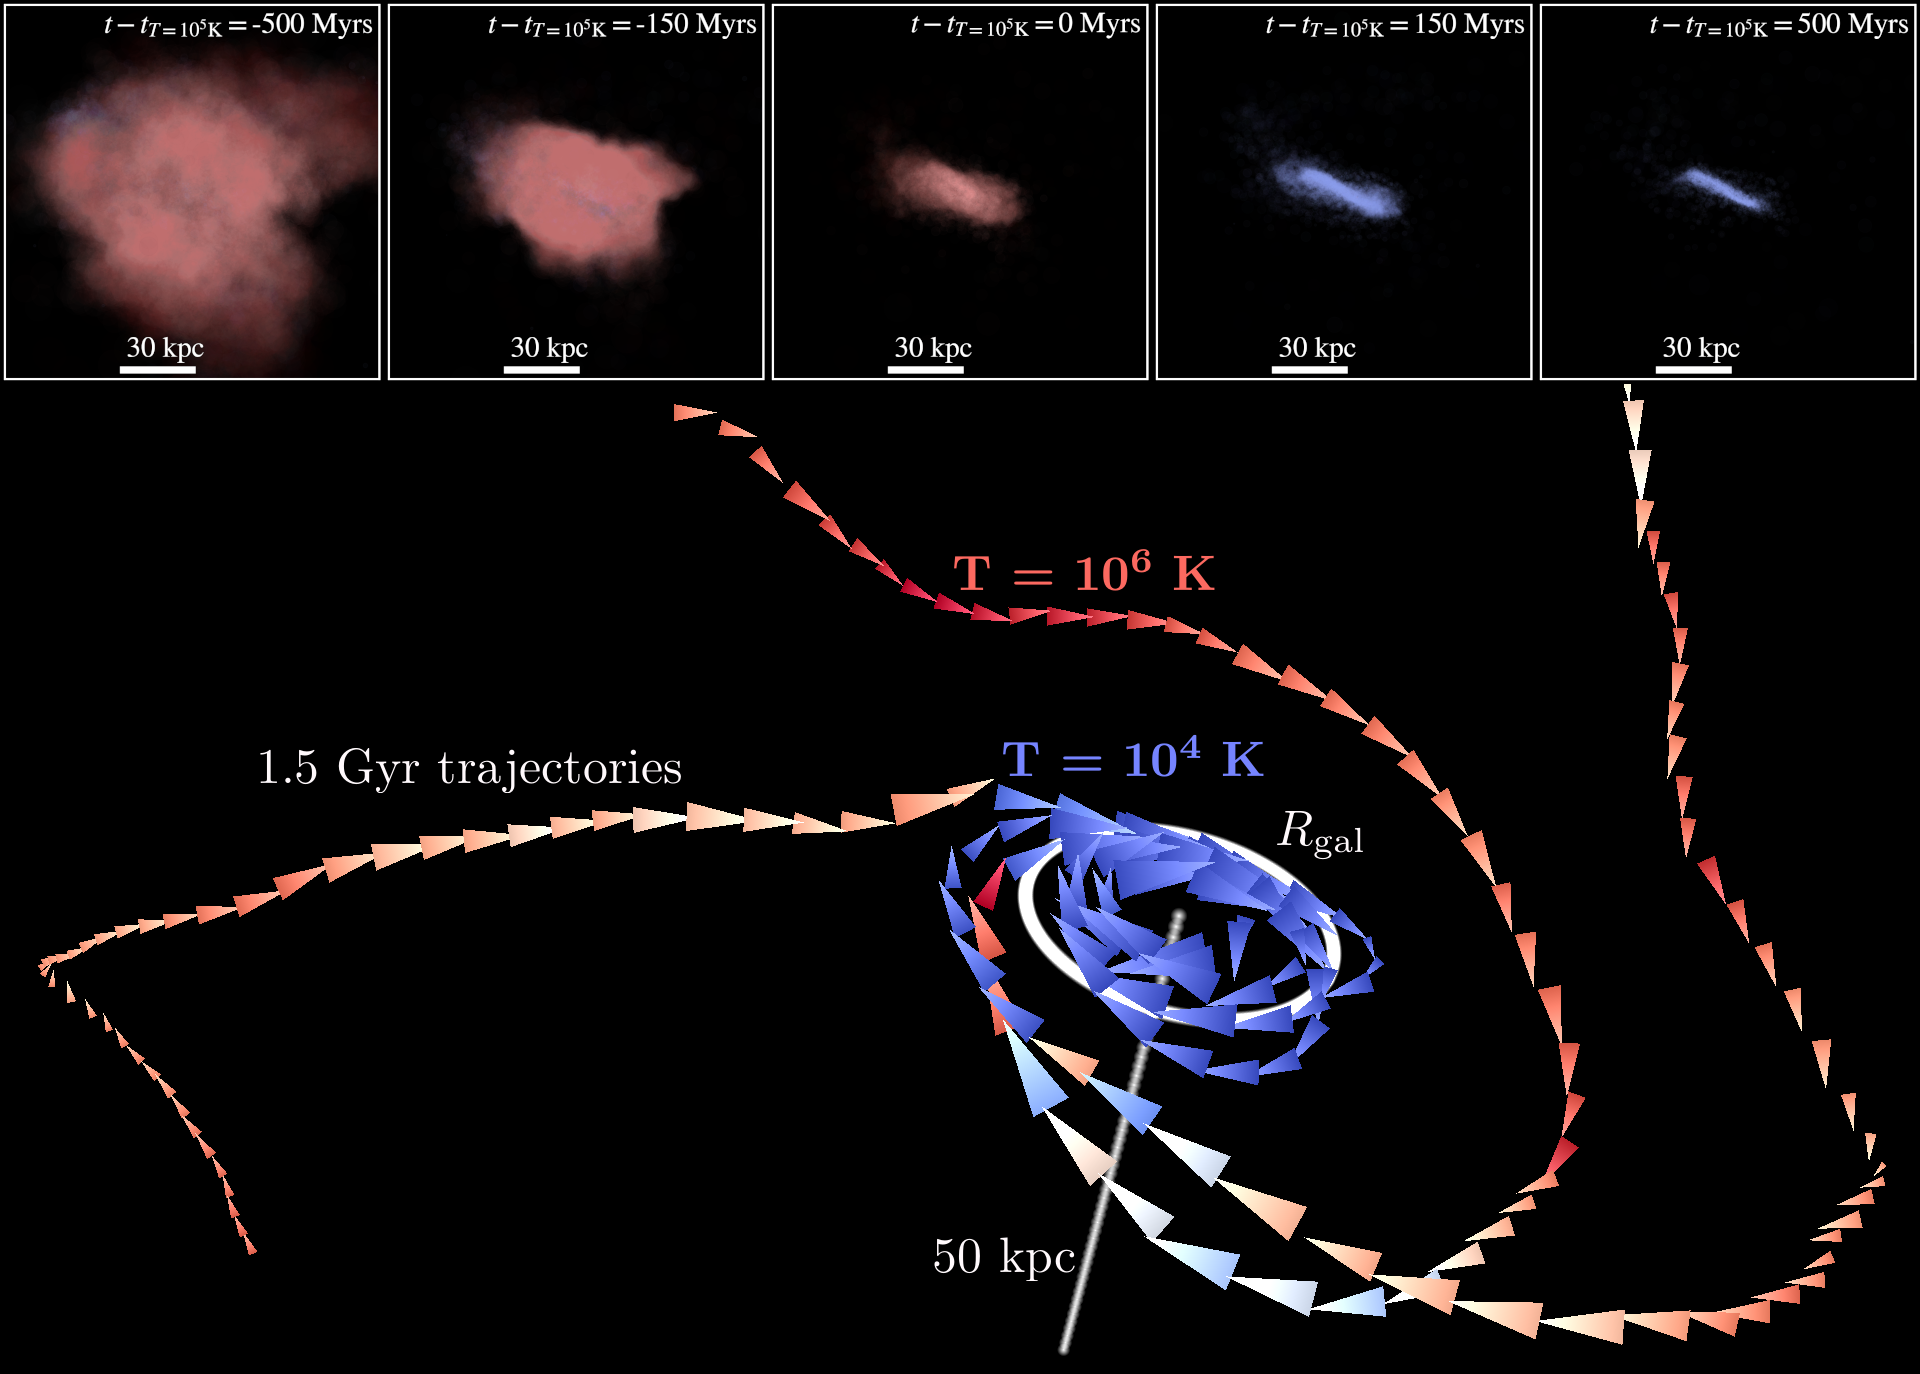
\includegraphics[width=\columnwidth]{figures/illustrative_tracks/illustrative_tracks.png}
    \caption{
Example trajectories showing how gas accretes onto Milky-Way mass galaxies at $z\approx0$.
Trajectories are representative trajectories selected from gas that is outside a Milky-Way-like simulated FIRE-2 galaxy one Gyr prior to $z=0$, and inside the galaxy at $z=0$.
We show the trajectories for 1 Gyr prior to the final time gas cools below $T=10^5$ K prior to accreting onto the galaxy, and 0.5 Gyr after cooling.
The trajectories are characteristic of \textit{quiet accretion}:
accretion that remains hot and voluminous until it cools at the galaxy-halo interface, at which time it becomes coherent and softly accretes onto the galaxy disk.
\textbf{
Consider adding additional complementary visualizations.
    }
    }
    \label{f: overview}
\end{figure}


% HOT IN HALO
\begin{figure*}
    \centering
    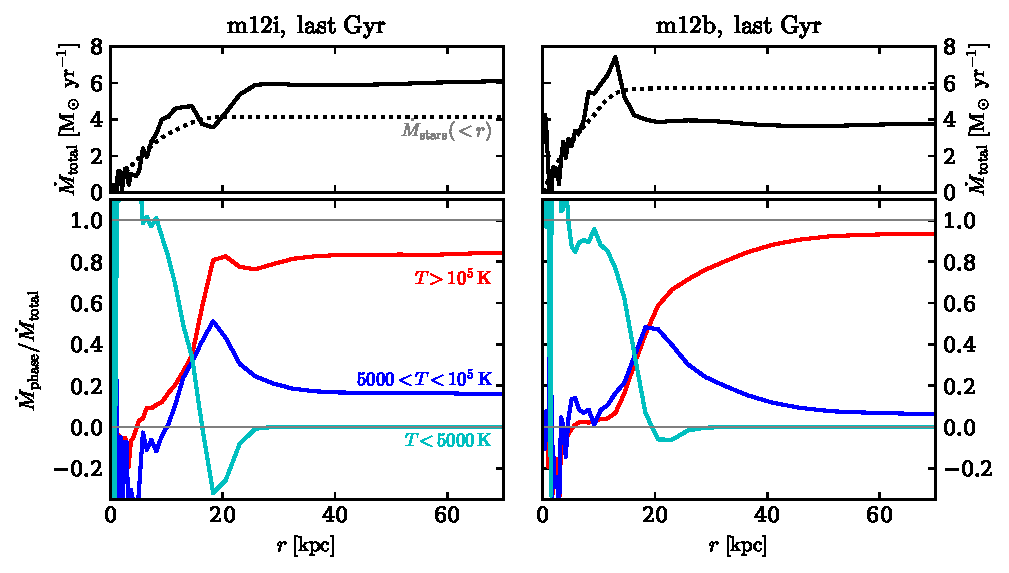
\includegraphics{figures/Mdot_normalized.pdf}
    \caption{
    Average mass inflow rate over the course of one Gyr prior to $z=0$ in two $L_\star$ simulated halos.
    Black lines in the top panels show the total mass inflow rate while colored lines in the bottom panels show the division into the hot, cool and cold phases. 
    The inflow is dominated by hot gas at $r\gtrsim 20 $ kpc, suggesting the dominance of hot mode accretion in these halos.
    For comparison the dotted line in the top panel shows the rate of gas conversion into stars within a given radius, and the radius at which it flattens indicates an edge to the galaxy.
    \textbf{verify conversion SFR to Mdot\_stars, add SFR of satellites}
    \textbf{Try adding labels relative to $T_{\rm vir}$ (Drummond's suggestion).}
    \textbf{Consider removing top panels, as scientists who are very aware of SFR discrepancies may become fixated.}
    % \textbf{Add images of face-on $z=0$ slice with temperature and velocity arrows.}
    % \textbf{Add top x-axis with radius in units of $\Rvir$}.
    % \textbf{Add cuts on density/temperature to avoid ISM gas causing a wide dispersion at low-r.}
    % \textbf{Change to linear space to emphasize halo. Cut out accretion shock.}
    % \textbf{Try using Clarke's entropy cut.}
    }
    \label{f: Mdot}
\end{figure*}

% COOLS AT DISK INTERFACE
\begin{figure*}
    \centering
    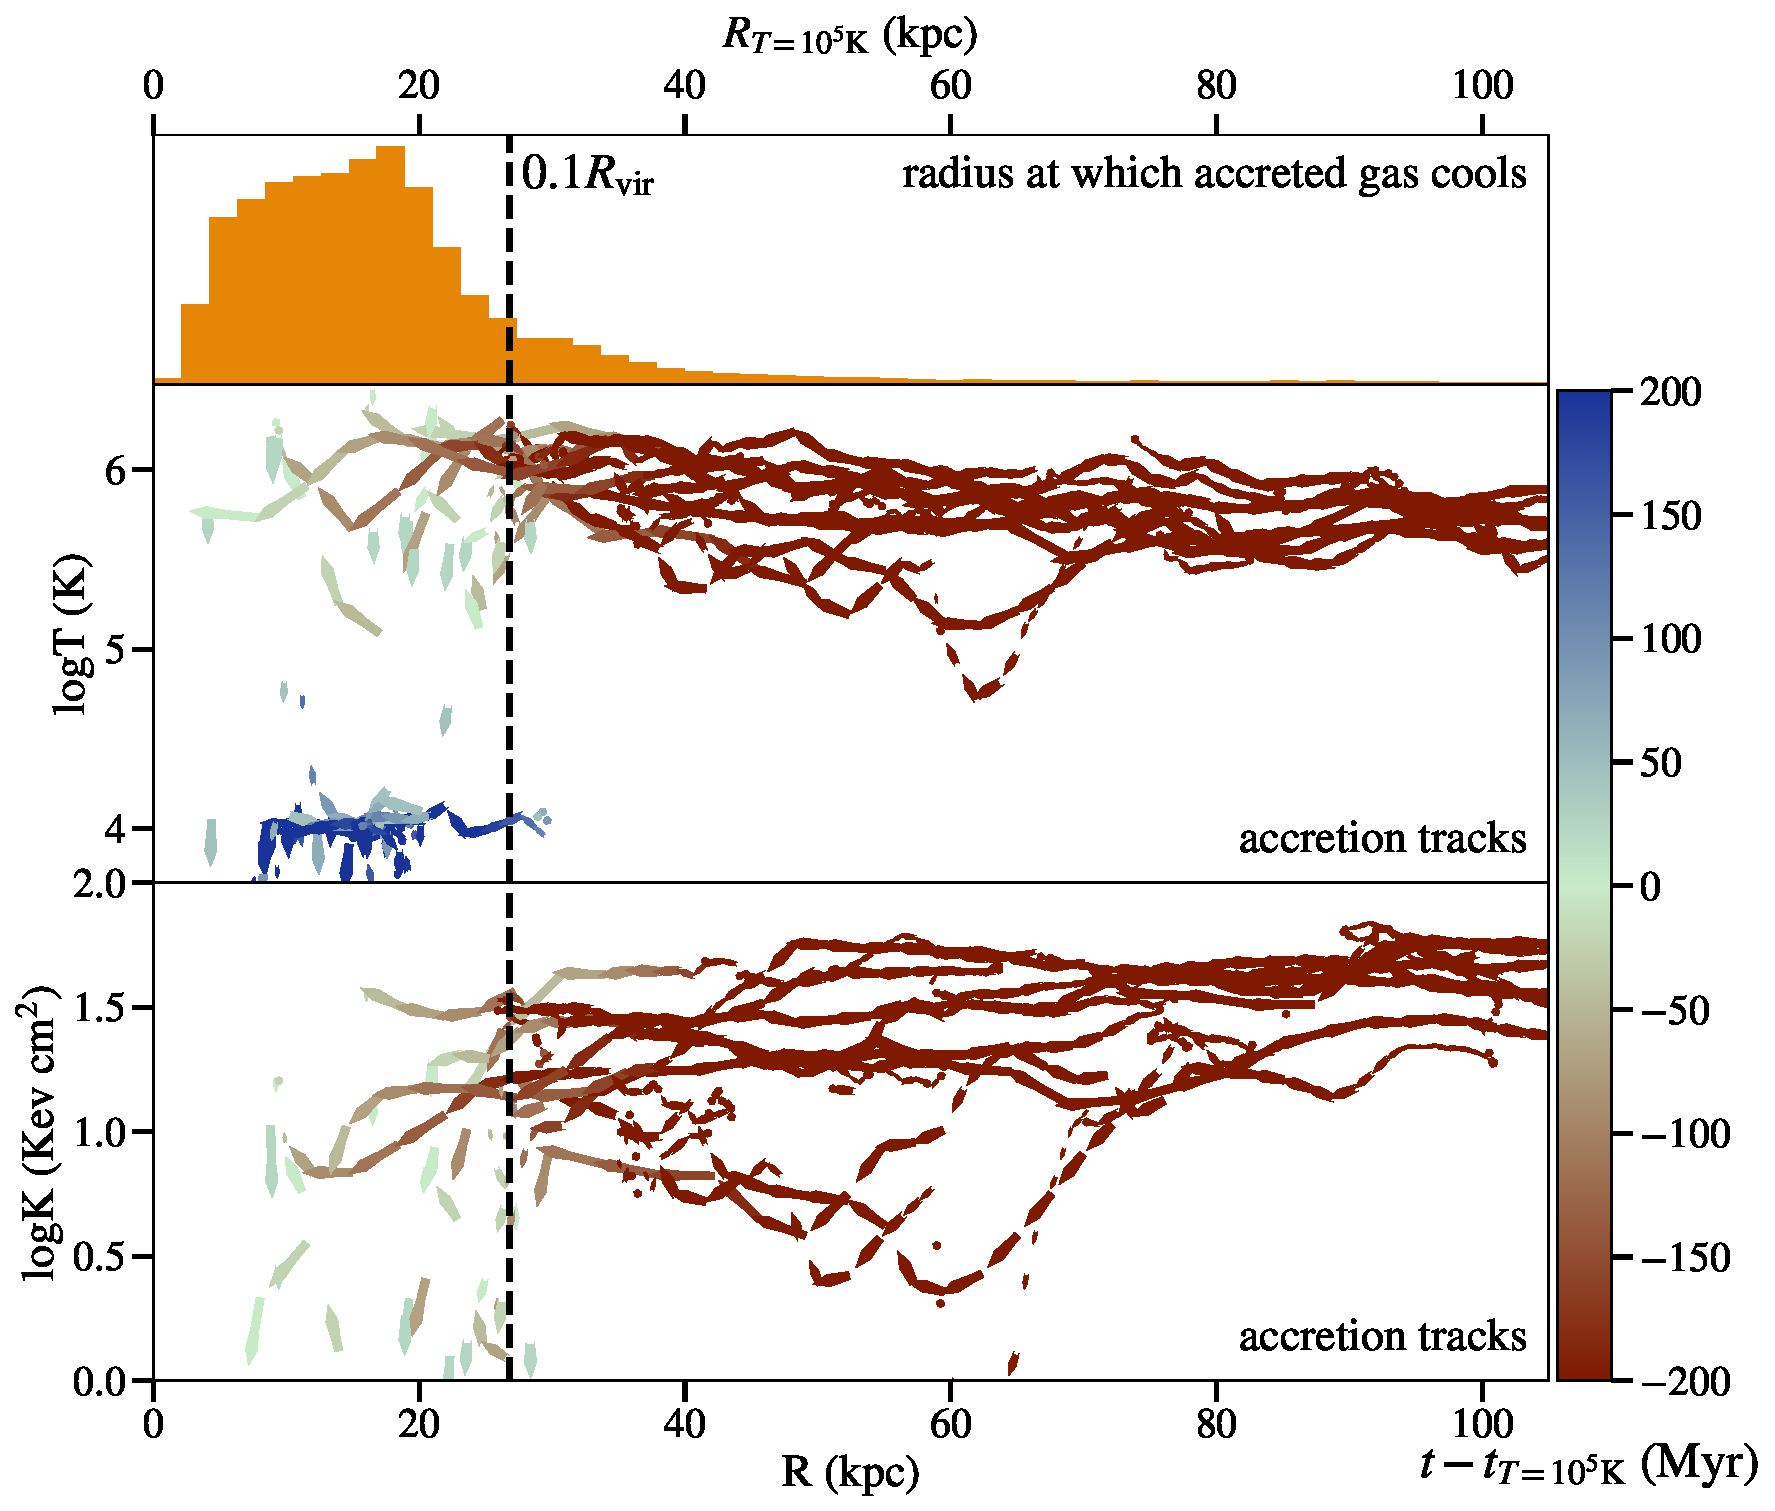
\includegraphics[width=\columnwidth]{figures/tracks_m12i_md.pdf}
    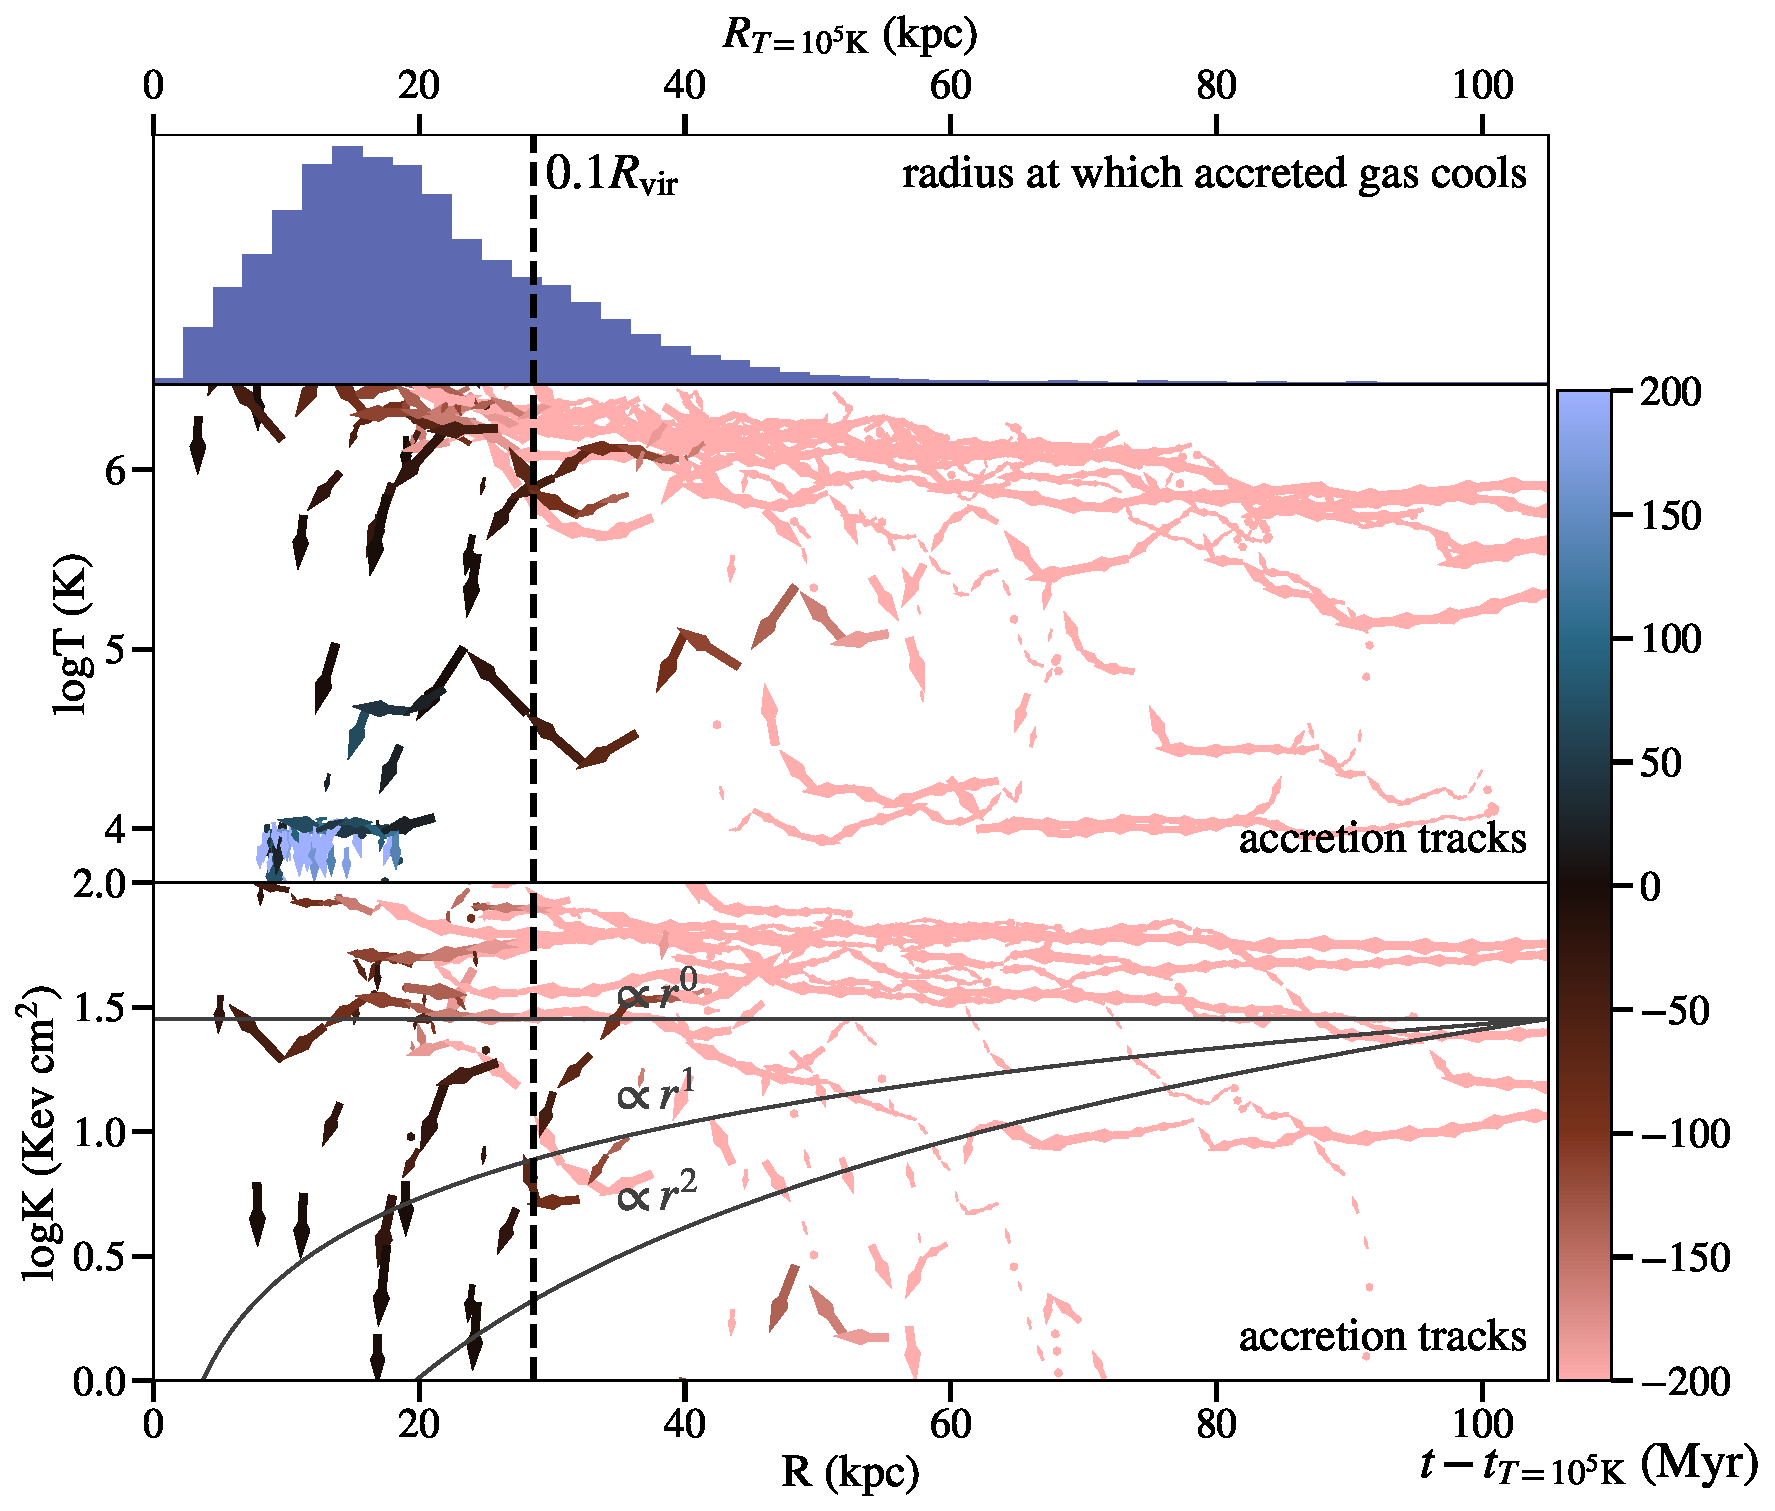
\includegraphics[width=\columnwidth]{figures/tracks_m12b_md.pdf}
    \caption{
    \textbf{Main panels:} 10 T vs.\ R and K vs.\ R tracks for two $L^\star$ halo at $z=0$, with color indicating time relative to the time at which gas cools.
    Gas either remains hot or cools only temporarily down to $\lesssim 0.1 R_{\rm vir}$. 
    % We do not show gas that has ever been ejected from the central galaxy.
    \textbf{Top panel:} Distribution of $\Rcon$, the radius at which gas particles last transitioned from $T > 10^5$ K to $T < 10^5$ K prior to accreting, i.e. the radius at which they cooled prior to accretion.
    \textbf{Try out fractional form: ultimate goal make it super clear (which the result is, so the presentation shouldn't hinder it).}
    \textbf{Remove vertical lines for Rsonic.}
    \textbf{Consider putting histograms by themselves to have a very simple, clear result with no distraction.}
    \textbf{
    Try plotting an edge-on image of the system to-scale above the histogram.
    }
    \textbf{
    Try making a 2D histogram of $\Rcon$ and the angle at which it accretes.
    }
    \textbf{
    What causes gas temperature to increase again after it reaches a low?
    In this random selection of ten particles at least 4 have a dip.
    }
 \textbf{Compare accretion radii (this plot) to a textbook angular momentum support radii distribution.}
 \textbf{Use R90 as the characteristic radii. See about using what someone else has derived.}
 \textbf{Show m11b histogram for comparison.}
    }
    \label{f: T vs R}
\end{figure*}

% ORIENTS AS IT COOLS
\begin{figure}
    \centering
    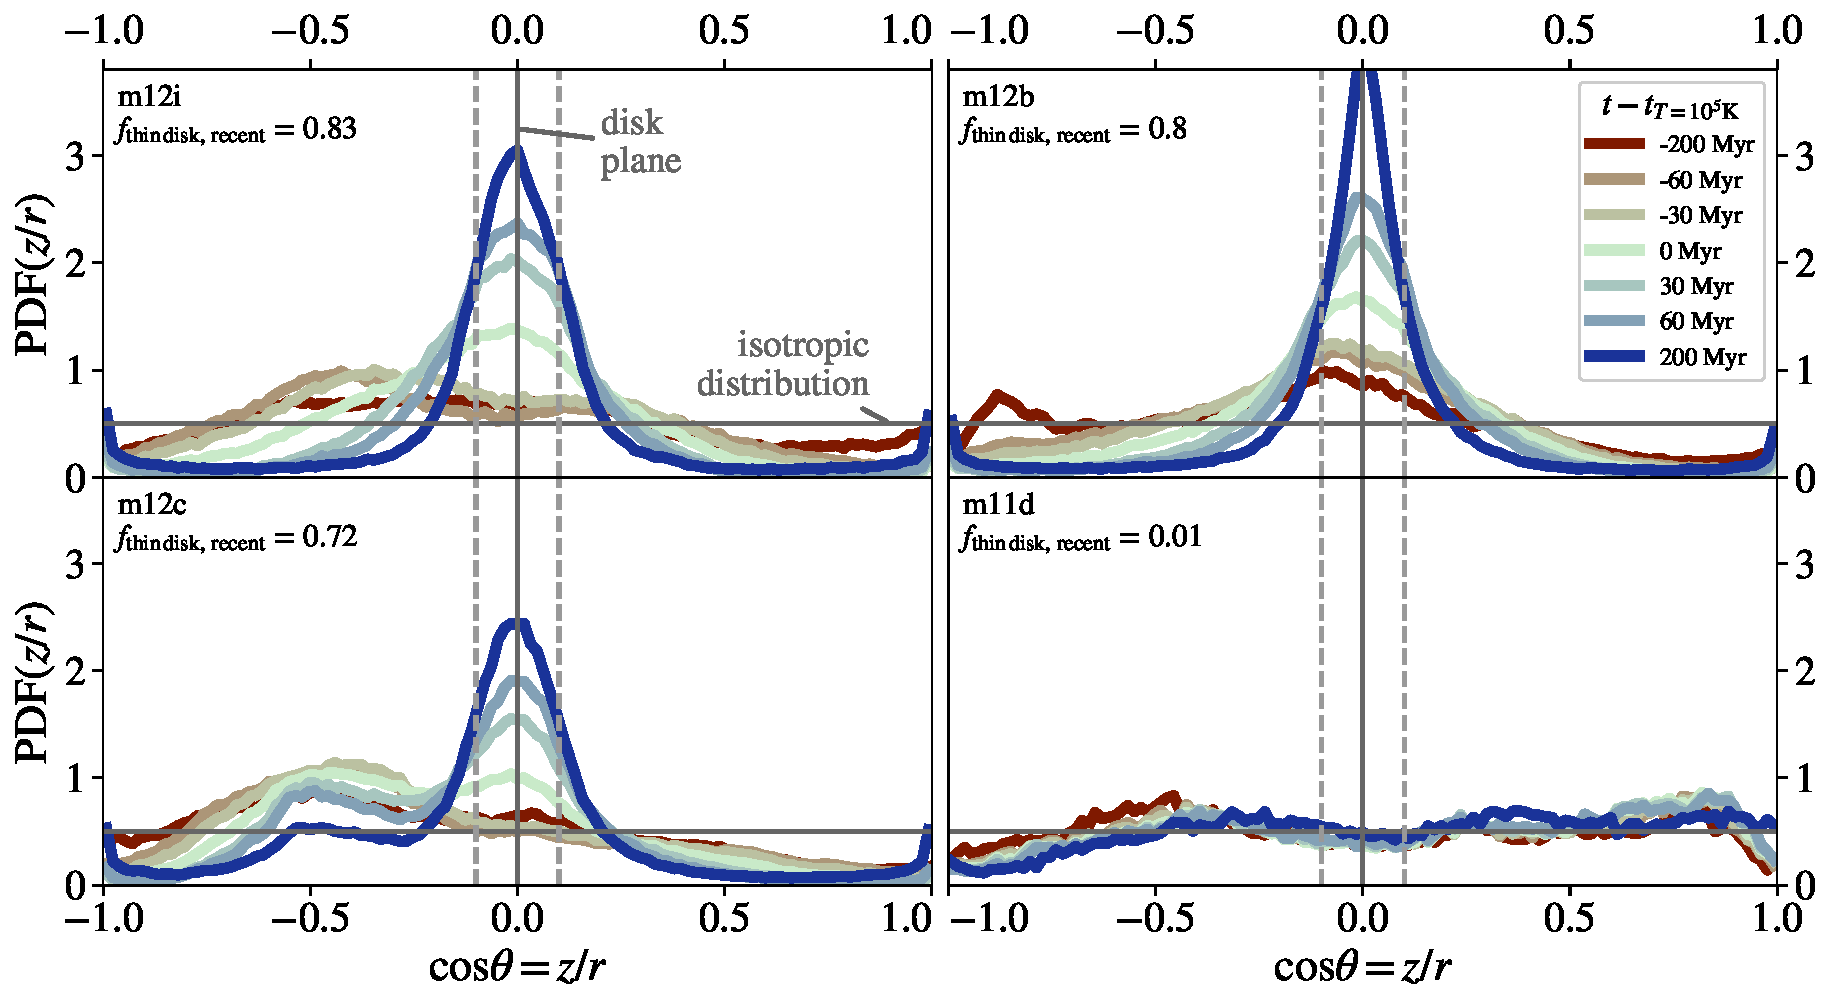
\includegraphics[width=\columnwidth]{figures/theta_vs_t.pdf}
    \caption{
    Angular distribution of accreting gas over 150 Myr before/after cooling. Cooling and circularization occur together -- prior to cooling the gas is distributed quasi-spherically, while after cooling the gas has a disc like configuration.
    \textbf{note `disc distribution' near vertical line'}.
    \textbf{Definitely m11d back in for comparison. An advantage for including is that it provides a powerful contrast.}.
    \textbf{Try splitting up into two panels side-by-side with a "before" panel and an "after" panel.}
    \textbf{Make a plot using the same particle bins as here, but showing the sum of the angular momentum for all particles in the bin, divided by vcR}
    \textbf{See if the distribution becomes narrower if selecting a narrower range of particles.}
    }
    \label{f: theta vs t}
\end{figure}

% MECHANICS OF QUIET ACCRETION
\begin{figure*}
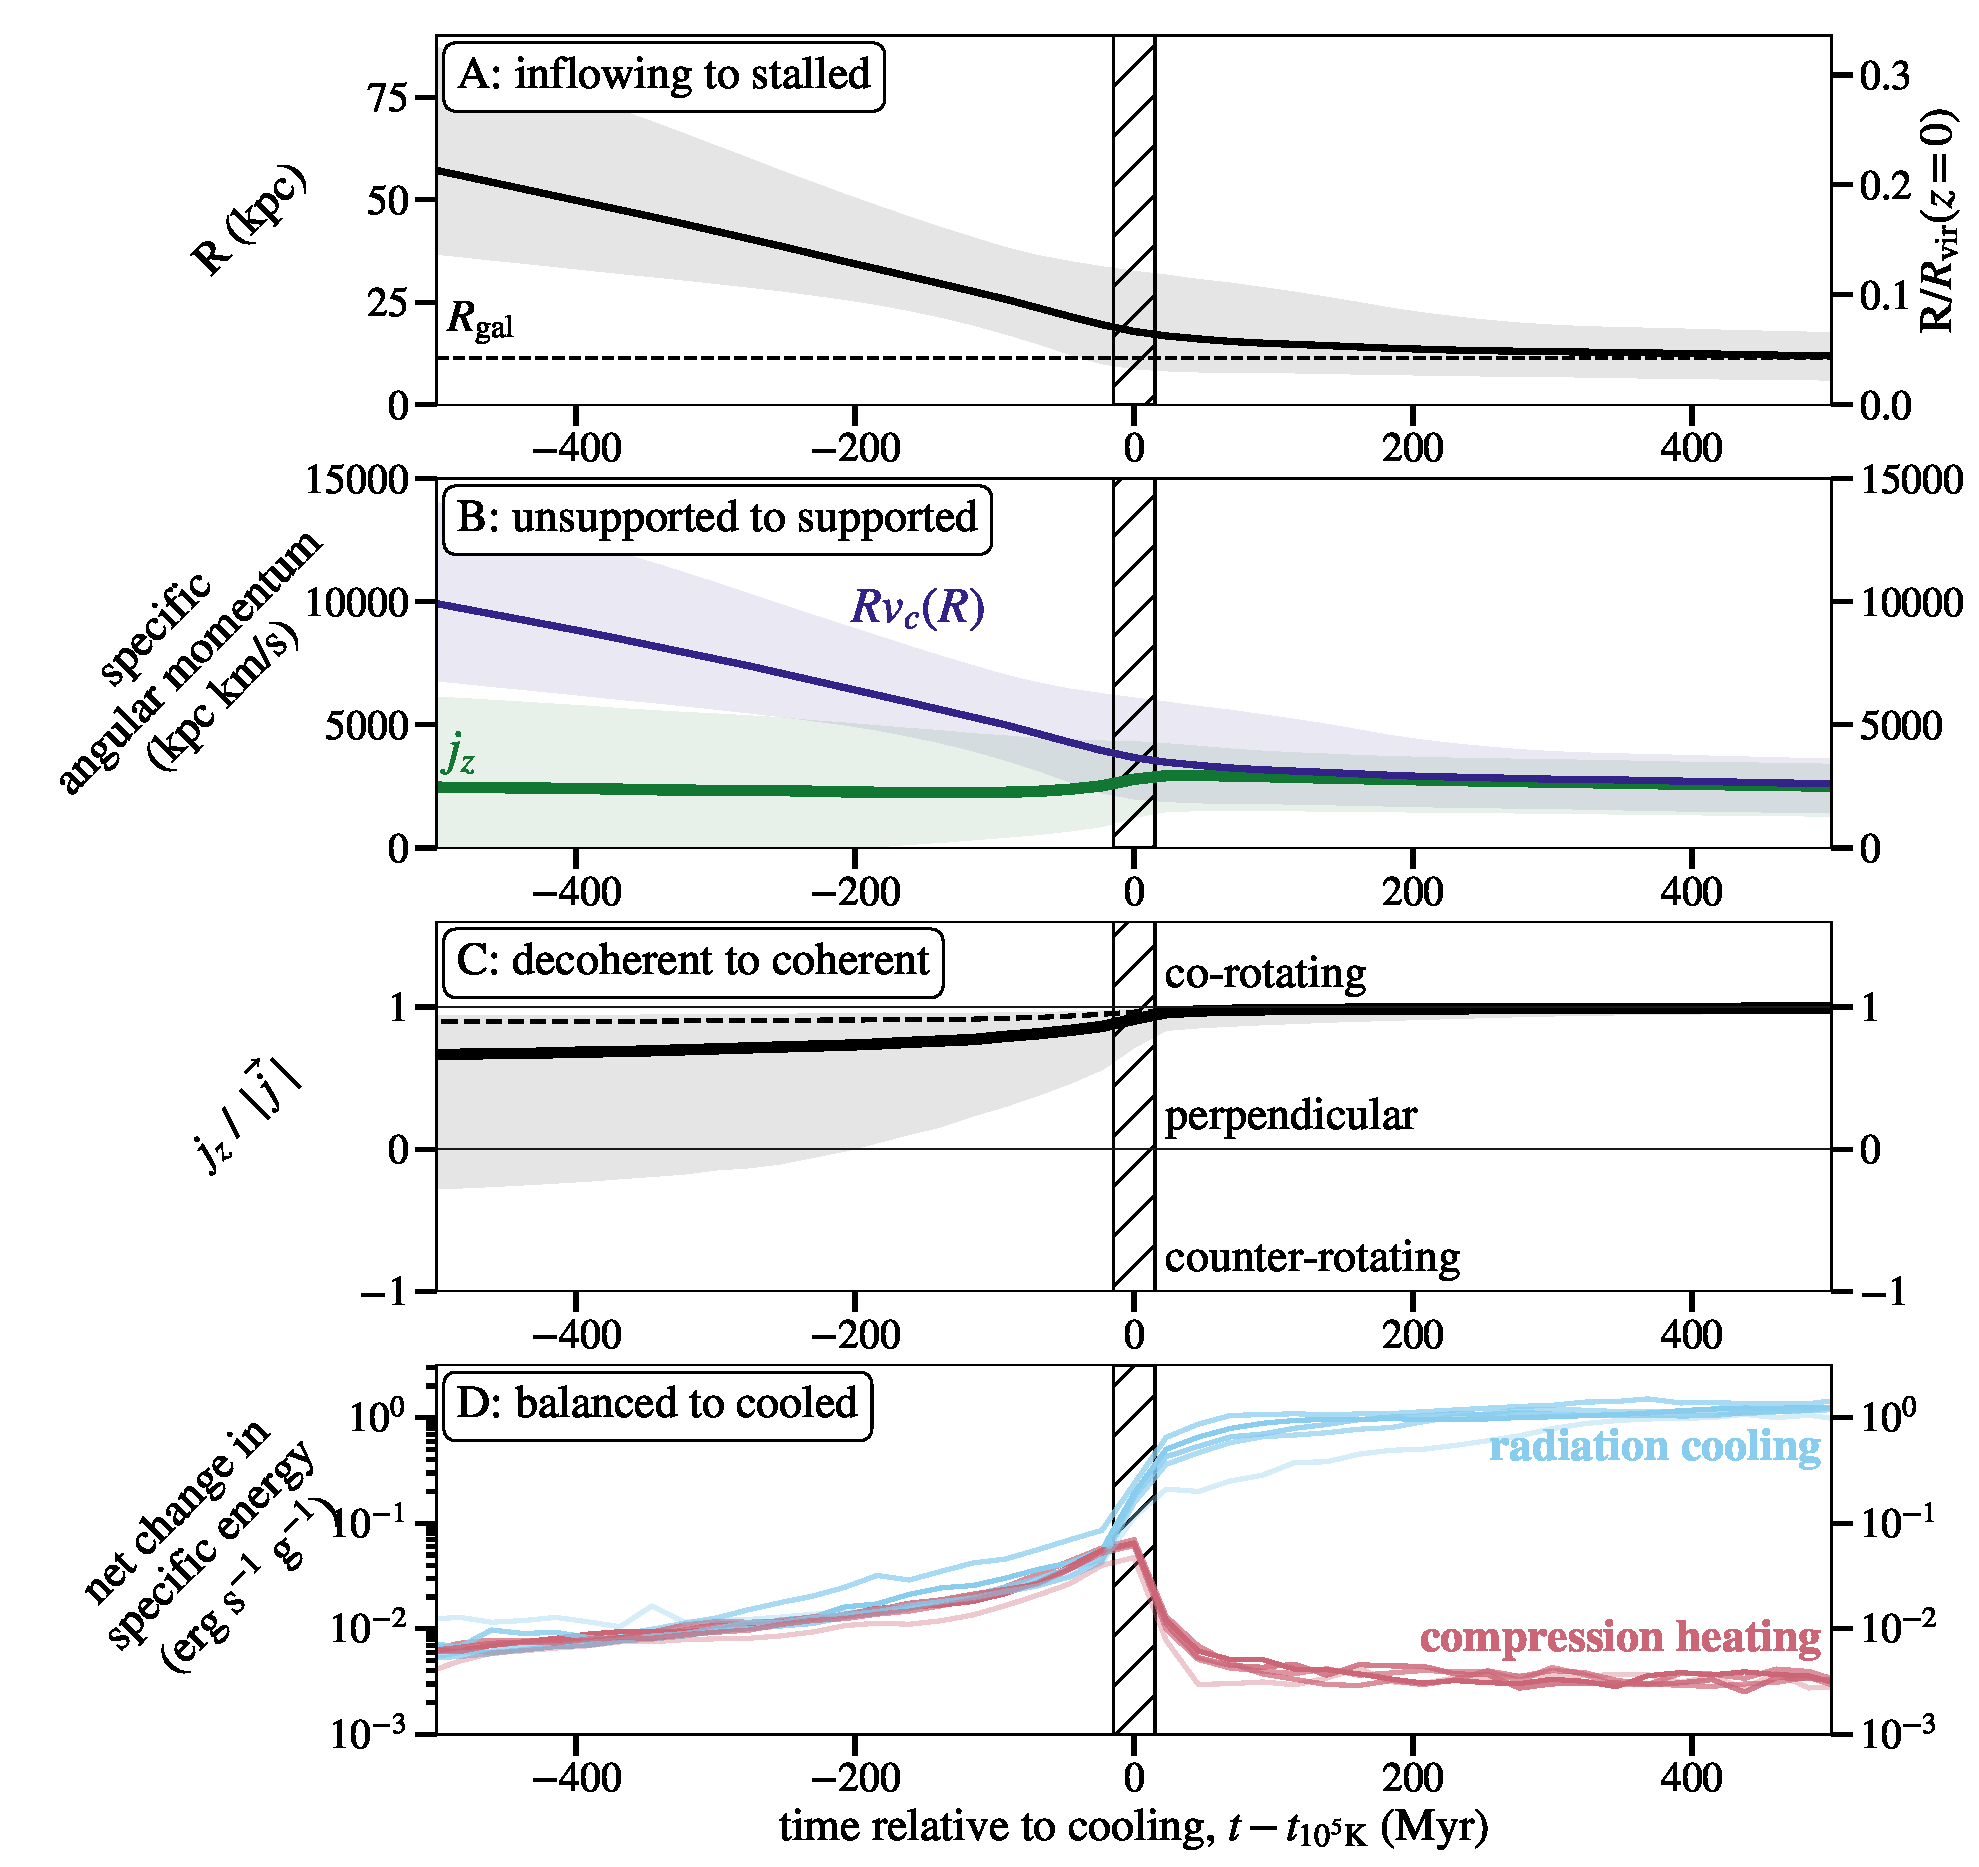
\includegraphics[width=\textwidth]{figures/before_vs_after.pdf}
\caption{
\textbf{Top:}
Radius versus time for 1 Gyr centered the time each individual particle cools ($t_{\rm 10^5 K}$).
Solid line is the median radius and shaded region shows the 16th to 84th interval among particles.
Gas moves inward smoothly until it cools, afterwards it moves inward much more slowly.
\textbf{Middle:}
Same as top but for the specific angular momentum of particles (green) and the the value of angular momentum needed to provide full rotational support ($Rv_c(R)$, purple).
Gas becomes fully rotationally-supported at the time it cools, contributing to the slower inward movement shown in the top panel.
\textbf{Bottom:}
Energy loss from radiative cooling (blue) and heating from $PdV$ work on the gas particles (red).
Each line represents the total change in specific energy for particles that cool at the same time (i.e. the same 100 Myr bin in $t_{\rm 10^5 K}$).
Prior to being rotationally-supported the gas cooling is offset by compressive heating, but lack of inward movement decreases the compressive heating afterwards while radiative cooling increases greatly due to increased density.
\textbf{
Try adding in m11 to see how it looks.
Emphasize these are particle tracks for accreting gas.
Address the increase in jz in panel two.Torquing of the disk? Collisional interaction, with evidence in the form of hot gas rotating slower?
Re: the hitch, it's crazy that anything could be that well-aligned cosmologically. The hitch could be pretty important in making the disk thin. Try remaking this plot in the thick disk phase.
The hitch may be driving inflow, because the disk could be giving angular momentum to it, allowing it to move in more.
Hint: the hitch is much less apparent in jmag.
Try showing for the fourth panel ( jvec - jz )/j, which we expect to go to zero, and shows the coherence and only the coherence pretty well.
Change tick labels in last panel.
}
}
\label{f: before and after}
\end{figure*}

% OBSERVATIONAL COMPARISON
\begin{figure}
\centering
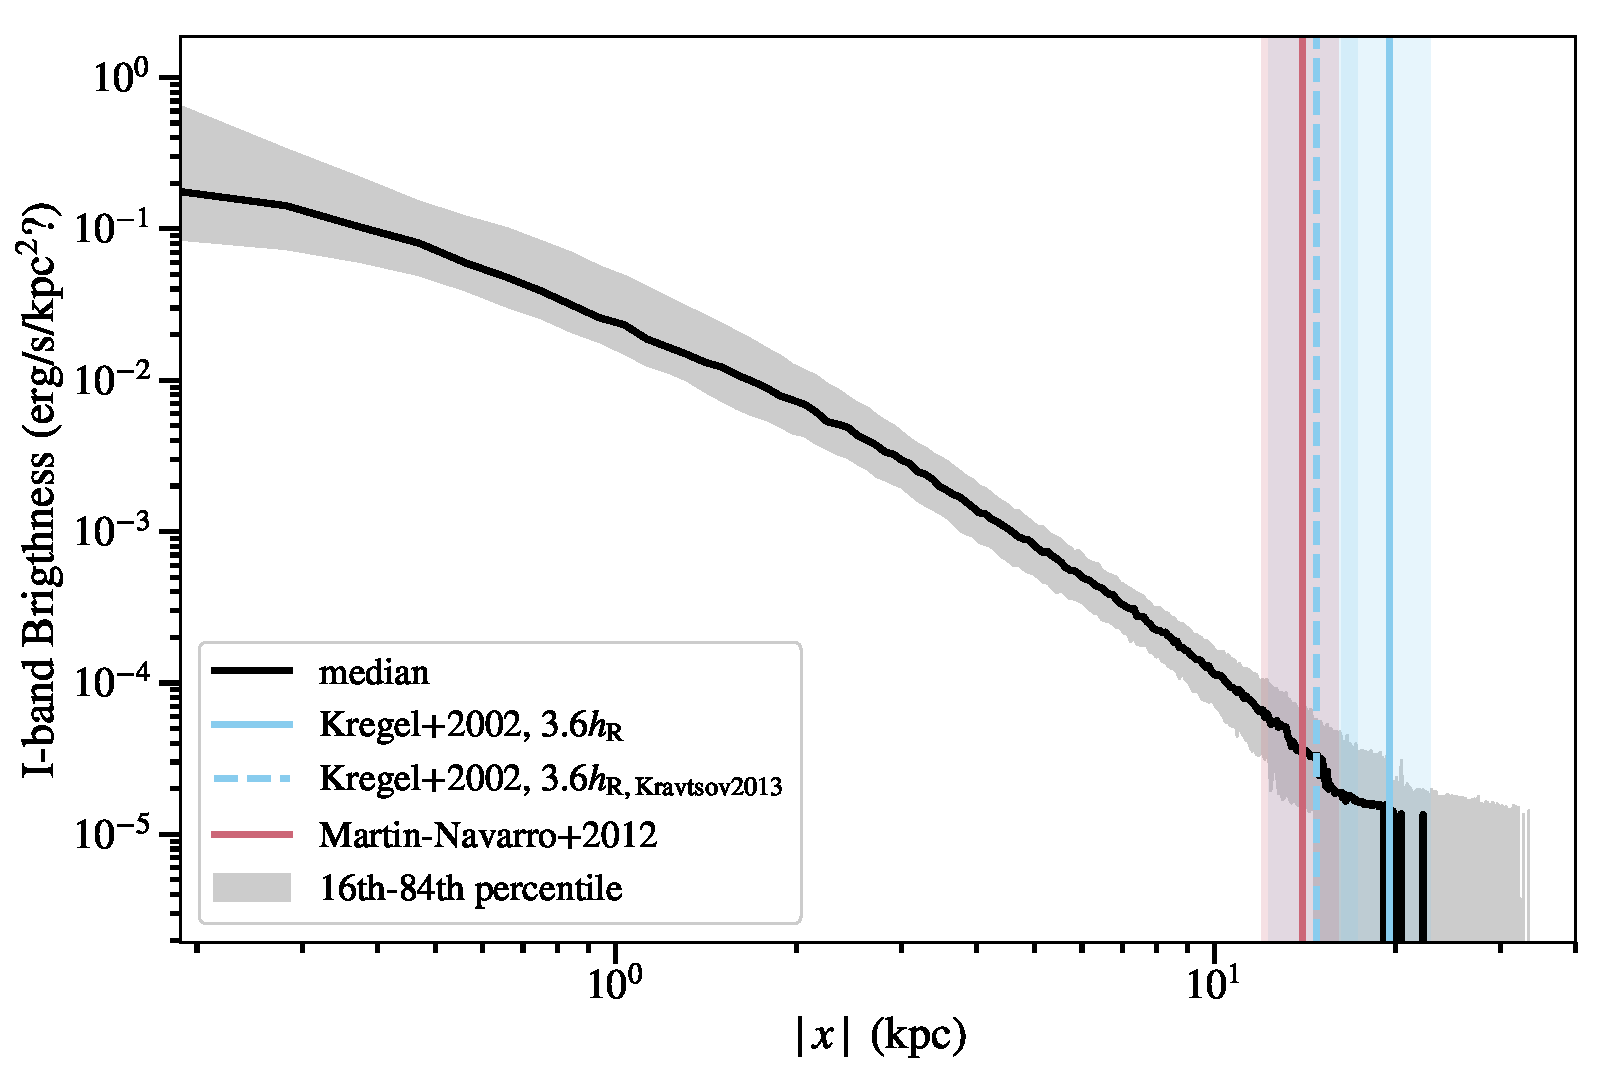
\includegraphics[width=\columnwidth]{figures/brightness_profile.pdf}
\caption{
I-band surface brightness profile for an edge-on stellar disk.
Black line (shaded region) is the median (16th-84th percentile) brightness among pixels 7.5 kpc above/below the disk.
The disk truncates at $\approx 12$ kpc, as seen by the sharp drop-off in the brightness for the percentiles, consistent with observations.
\textbf{
Fill out observations description.
Put on log-linear axis.
Cut out inner radii where dust obscuration is likely an issue.
Maybe cut out entirely and just reference Cameron's paper.
Reference Shea and Kareem's papers.
}
}
\label{f:stellar_profile}
\end{figure}

% SPARE FIGURE
\begin{figure}
    \centering
    % \includegraphics{}
    \caption{
    \textbf{Spare figure, but maybe
    cooling emission in X-ray, optical and UV lines vs.\ radius, only from tracked particles
    }
    }
    \label{f: emission}
\end{figure}

\section{NOTES FOR AUTHORS}

\subsection{KEY FOR COAUTHORS}
\textbf{Bold: Notes for things to implement.} \\
\textit{Italics: Rough text, needs polishing.} \\
Normal: Normal text, polished enough to be included in a draft.

\subsection{OUTSTANDING QUESTIONS/DISCUSSION POINTS}

% Target audience
\textbf{
The target audience is:
At the broadest level anyone who wants to understand the general picture of how disks form.
Galaxy theorists.
CGM theorists.
Galaxy observers.
CGM observers.
People who like interpretable results.
}

% Assess the overall message
\textbf{
Imagine sitting down with the target audience.
What are the most important points you want to convey?
In particular, what could they really use?
Think first and foremost of that, and shape accordingly.
}

% Review
\textbf{
Read through the paper with each targeted group in mind.
Edit accordingly.
Even better, get a member of the target group to provide feedback.
}
\textbf{
At the end, decide on the title and the abstract.
}

% Temporary cooling investigation
Some trajectories cool and then reheat shortly before accreting, check why.
Why is there cool gas visible in the intuition-building plots 100 Myr prior to cooling?

% Additional simulation analysis questions
Why do m12f and m12r have a very extended distribution of $\Rcon$?
Why does m12f have increasing diskiness as it cools, but it starts from already being disky?
Why does m12r have no change in angular distribution?

% How much to include on CR sims
Pros of including CR-analysis:
- The physical mechanisms do not require the halo to be a classic virialized hot halo.
- According to our three characteristics that define quiet accretion, quiet accretion is observed in CR simulations.
- Quiet accretion is a more interesting concept if we point out its generality.
- Cameron Trappe also wrote a paper, and one of the main differences is the inclusion of cosmic rays. I'm not sure there's room to do a third entirely separate paper on cosmic ray quiet accretion. Most things will have been covered.
- As an extension of the previous point, because Cameron wrote the CR paper we can just include a single plot or so and point to his paper for the details of how accretion works.
Cons:
- CR halos are regarded as fundamentally different to hydro halos
- Jonathan's previous work doesn't touch on CR halos.

% Summary plot
Metric of diskiness vs metric of quiet accretion.
Quiet accretion metric: violin plot/median of $\Rcon$.

% Check my definition
First vs last time cooled.
Dependence on galaxy density criterion.

% Name: Quiet accretion?
Is quiet accretion the term we want to use?
Use inspiration from the pre-virilization comparison.
Alternatives:
Soft, soft-landing.
Slow?
Gentle?
Spiraling?
Sharp? (Sudden and ubiquitous at angular momentum support radius.)
Write to Mary Putman and ask why she called it quiet accretion.

% CRs or no?
Do we want to include CRs in this paper?
If including, plot temperature distribution while tracking to compare and contrast CRs and non-CRs.
When doing CR-comparison panel overplot fiducial simulation results.

% Check differentation of definition and results
When presenting we should ensure we're clearly differentiating definition and results.

% Not overly centered on disk formation
Framing of conducive to disk formation might give your listeners the impression that this is the only theory for disk formation.

% Outer virialized halo effects
Check the following picture, suggested by James:
Far enough out in an m11 the inner halo is virialized, and compressive heating can contribute comparably to cooling.
This would suggest the cooling radius is max( edge of the virialized area, angular momentum radius), potentially true across all halo masses MW and below.
Can be checked by making an equivalent to Figure~\ref{f: before and after} for an m11.

% Firefly changes
Good preset. Requires changing using options. Can load a preset using the Options class.)
Change loading screen.
Include labels for scale.

% Plots for a future observational paper
Multi-panel image:
HI-weighted row,
OVI?-weighted row,
T-colored row.
Before column(s), at column, after column.
Try mollweide projection.
Try classic kinematic picture showing blue/red-shift along LOS.

% Misaligned or warped disks
Can quiet accretion produce misaligned or warped disks?
Tjitske has seen in large scale simulations a misaligned disk being preceeded by a change in halo angular momentum.
Anna has some plots of this. This might be more present in the ELVIS sims.
The angular momentum vector of the CGM is in general misaligned with that of the stars in the central galaxy by large angles  30 to 60 degrees (DeFelippis et al. 2020).
See also Roskar2010.

\section{Introduction}
\label{s: introduction}

% Star formation and CGM accretion
\textit{
Star formation on a galactic scale informs the distribution of formation times for systems ranging from stellar populations~\cite{Yu2021} to star clusters~\citep[e.g.][]{Grudic2020} to planets~\textbf{find citation}.
In this way galactic star formation is one of the main intersections between many fields of astrophysics.
Galactic star formation is itself informed by accretion from the circumgalactic medium (CGM) that surrounds galaxies.
This accretion from the CGM provides fuel without which star formation would cease in only a couple of Gyrs~\cite[e.g.][]{Prochaska2009, Bauermeister2010, Spring2017}.
}

% Cosmological simulations
\textit{
Modern cosmological simulations provide a means to understand the prevalence, mechanics, and characteristics of different accretion modes.
These simulations include a combination of cosmological environment and galactic physics, which has allowed simulators to investigate accretion while accounting for both its cosmological nature and its interaction with galaxies and their CGM~\citep[e.g.][Trapp et al,. in prep.]{Oppenheimer2010, Stewart2011, Fernandez2012, Ford2014, Angles-Alcazar2017, Hafen2019, Hafen2020, Ho2019, Rottgers2020}.
Of special note are ``zoom-in'' simulations that focus on resolving a single halo and its environment, enabling high resolution while preserving cosmological structure~\citep[e.g.][]{Katz1993, Hopkins2014, Hopkins2018, Wang2015, Agertz2020}.
The FIRE simulations~\citep{Hopkins2014, Hopkins2017}\footnote{\url{https://fire.northwestern.edu/}} are a set of zoom-in simulations that resolve stellar feedback on the scale of giant molecular clouds in the ISM, producing winds that naturally expand into the CGM and interact with accreting gas~\citep{Muratov2015,Muratov2016, Hafen2019, Hafen2020}.
The resultant galaxies are broadly consistent with the stellar mass-halo mass relation~\citep{Hopkins2017}, the mass-metallicity relation~\citep{Ma2015}, satellite galaxy populations~\citep{Wetzel2016,Garrison-Kimmel2019a}, and can have thin-disks consistent with Milky Way-like galaxies~\cite{Garrison-Kimmel2018, El-Badry2018}.
}

% Accretion types - cool
\textit{
There are believed to be a number of modes of accretion from the CGM, each with different characteristics, mechanics, prevalences, and affects on galactic star formation.
One canonical accretion mode is cool, filamentary accretion, wherein cool, $T \sim 10^4$ K cosmological filaments travel into the galaxy  from the IGM~\cite[e.g.][]{Keres2005, Dekel2006, Keres2009, Martin2019a}.
Filamentary accretion is especially relevant at high redshift when the universe is denser~\citep[e.g.][]{Keres2009a, Stern2019, Huscher2020}.
Filamentary accretion can often be accompanied by ``clumpy'' accretion in the form of accreting satellite galaxies and their CGMs~\citep[e.g.][]{Hafen2019, Hafen2020}, which in some cases can provide fuel that produces more than a third of stars formed in MW-mass galaxies~\citep{Angles-Alcazar2017}.
}

% Accretion types - hot
\textit{
For Milky Way-analogs, hot gas with temperature $T>10^5$ K dominates the inflow of gas, as found commonly by cosmological simulations~\citep{Faucher-Giguere2011a, VandeVoort2011, VandeVoort2012a, Joung2012, Murante2012, Nelson2013}.
One such accretion mode is instability-driven accretion, wherein gas precipitates out of the halo due to hydrodynamic instabilities~\citep[e.g.][]{Maller2004, Mccourt2012, Voit2015, Armillotta2016, Gronke2019a, Esmerian2020, Voit2021}.
}

% Quiet accretion
\textit{
Another type of hot accretion is ``quiet'' accretion, wherein the accreting gas remains hot down to the galaxy-halo interface, at which time it cools and accretes onto the galaxy~\citep{Putman2012}.
Consistent with a quiet accretion mode, some observations detect ionized, inflowing gas at the galaxy-halo interface~\citep{Zheng2017}.
Previous idealized simulations have simulated cool gas clouds condensing onto galaxies and found that disrupted and heated clouds could condense and cool at disk edge~\citep{Heitsch2009}.
However, to-date little work has been done to distinguish how prevalent quiet accretion is in a cosmological environment and the detailed mechanics of how it proceeds.
}

% This paper
\textit{
In this paper we show that quiet accretion is the primary mode of gas accretion onto central Milky Way-mass galaxies at $z \sim 0$ in the FIRE simulations.
In \S\ref{s: characteristics} we show that the vast majority of accreting gas has characteristics consistent with quiet accretion.
In \S\ref{s: mechanics} we analyze the mechanics through which quiet accretion occurs.
In \S\ref{s: other modes} we compare quiet accretion as seen in our simulations to other accretion modes.
In \S\ref{s: prevalence} we discuss the prevalence of the quiet accretion mode, focusing on the conditions that enable quiet accretion, including an equivalent mode in halos with non-thermal support.
In \S\ref{s: fueling} and \S\ref{s: disk formation} we discuss the implications of quiet accretion for fueling star formation and encouraging disk formation, respectively.
We offer some brief insight on observational expectations for quiet accretion in \S\ref{s: observational expectations} before concluding in \S\ref{s: conclusions}.
}

% % Angular momentum theoretical estimates
% \textbf{
% Filippo's collaborator work: https://ui.adsabs.harvard.edu/abs/2017MNRAS.467..311P/abstract
% }

% % Observational evidence
% \textbf{
% Reaches back to Barcons+1995: https://www.nature.com/articles/376321a0.
% See also Yong+2017ab.
% \url{https://ui.adsabs.harvard.edu/abs/1995Natur.376..321B/abstract}
% \url{https://ui.adsabs.harvard.edu/abs/2013Sci...341...50B/abstract}
% \url{https://ui.adsabs.harvard.edu/abs/2016ApJ...820..121B/abstract}
% \url{https://ui.adsabs.harvard.edu/abs/2019MNRAS.485.1961Z/abstract}
% \url{https://ui.adsabs.harvard.edu/abs/2017ApJ...835..267H/abstract}
% Bielby et al. 2017; Péroux et al. 2017; Diamond-Stanic et al. 2016; Muzahid et al. 2016
% Wong et al., 2004; Martin et al., 2012; Rubin et al., 2012; Ho \& Martin, 2020
% Zabl 2019
% Zheng2017
% }

% % C-A comments
% \textbf{
% Galaxies have lower j than the CGM due to preferential accretion of low-j gas.
% Low angular momentum gas is more likely to form stars because it moves inwards and increases density.
% https://ui.adsabs.harvard.edu/abs/2019MNRAS.488.4801J/abstract
% https://ui.adsabs.harvard.edu/abs/2015MNRAS.449.2087D/abstract
% this paper also discusses/assumes low sAM gas preferentially ends up in stars:
% https://ui.adsabs.harvard.edu/abs/2017MNRAS.466.1625Z/abstract
% }

% Jonathan Info dump
% Some refs on truncation radius in observations:
% \cite{Kregel2002} tight correlation between disk truncation radius and Re (Spearman 0.95) in 34 edge-on spirals (in face-on galaxies stellar halos can outshine truncation, see Martín-Navarro+14). $R_{\rm truncation} / R_e({\rm Iband}) \sim~ 3.6$. Somewhat higher ratio in small Re spirals, somewhat lower ratio in bluer passbands (where Re is larger).
% Re is independently found to be proportional to the virial radius, roughly Re ~ 0.015 Rvir (e.g. Kravtsov13).
% Martín-Navarro+12: 34 edge-on spirals from SDSS / S4G: Rtruncation ~ 1.1 R25, where R25 is the radius at which the surface brightness equals 25mag
% van der Kruit+07: when a HI-warp is present in the gaseous disc it starts at 1.1 Rtrunc; the truncation radius and the onset of the warps coincide radially sometimes with features in the rotation curve and often with steep declines in the HI surface density; inner disks are very flat and the onset of the warp just beyond the truncation radius is abrupt and discontinuous;
% Perez+04, Trujillo\&Pohlen05, Azzollini+08: measurements of truncation radius at z~1
% Comeron+12: 70 edge-on S4G galaxies. 77\% of thin discs truncate, but only 31\% of thick discs. $M_thick/M_thin$ increases with decreasing $v_c$
% de Jong+07: Stellar Populations across the NGC 4244 Truncated Galactic Disk
% Haberzettl+07: truncation in LSBs
% some suggested theoretical explanations of breaks:
% https://ui.adsabs.harvard.edu/abs/2009MNRAS.398..591S/abstract
% https://ui.adsabs.harvard.edu/abs/2008ApJ...675L..65R/abstract
% https://ui.adsabs.harvard.edu/abs/2006ApJ...645..209D/abstract
% https://ui.adsabs.harvard.edu/abs/2009ApJ...705L.133M/abstract
% https://ui.adsabs.harvard.edu/abs/1987A%26A...173...59V/abstract
% and short summary sentence from Comeron+12 intro:
% "Several theories compete for explaining the origin of such breaks. Truncations have been explained by dynamical arguments related to the conservation of angular momentum during galaxy formation, by star formation thresholds, and by the redistribution of angular momentum by a bar. Antitruncations have in some cases been linked to interactions and mergers."
% Antitruncations are cases where the Surface Brightness profiles flattens at large disc radii rather than steepens. From my impression of the observational literature anti-truncations are seen mainly in face-on galaxies and are related to the existence of stellar halos

% \textbf{
% Misc notes from Halo21
% Norbert Werner sees the X-ray atmosphere is flattened, along the disk.
% Mark Voit: complementary view is that rotation destabilizes halo gas.
% Sormani and Serbachi idealized rotating hot halos.
% Oppenheimer rotating hot halo.
% }

% % Observational inflow evidence
% \textbf{
% Hwang, Barrera-Ballesteros, Heckman+2019: ``anomalously low-metallicity regions'' in MaNGA galaxies in $\sim 25\%$ of MaNGA SF galaxies. Luo, Heckman+2021 is a follow-up.
% Howk, Rueff, Lehner+2018: extraplanar gas is lower metallicity.
% Putman, Peek,\& Joung 2012, Putman review for HVCs, best fit inflow speeds are -40 km/s, predict accretion rate of $\sim 0.1 M_\odot/$ year (with correction factor multiplied by two for ionized component; Lehner\&Howk 2011).
% IVCs: Rubin+2019 is a good start, Richter+2017 provides a review.
% Bregman hot halo rotation (cited by Ben).
% }

% % Radial Inflow
% \textbf{
% Observational estimates of disk rotation:
% https://ui.adsabs.harvard.edu/abs/2004ApJ...605..183W/abstract
% https://ui.adsabs.harvard.edu/abs/2019ApJ...883...77S/abstract
% }

% \textbf{Just go through Crystal Martin's Halo21 Keynote...}

% \textbf{The accretion isn't completely polar symmetric.}

% \textbf{Galaxy size and relation to angular momentum:
% https://ui.adsabs.harvard.edu/abs/2017rlbc.confE..29K/abstract}

\section{Methods}
\label{s: methods}

% Simulation sample
\textbf{Waiting for the analysis to finish running on the additional simulations to fill this in.}
\textbf{Also do massive galaxies?}
\textbf{Do more metal diffusion simulations (the non-md sims have unexpected cooling at large radii): at least 4 metal diffusion simulations would be good.}

% Metal diffusion
\textit{
The metal distribution in the CGM affects cooling processes and therefore the treatment of metal diffusion is important for resolving substructure and small clouds~\cite{rennehan2021}.
More diffusive metal diffusion typically produces less substructure, with possible exceptions for stripping processes, and many current prescriptions for metal diffusion may under-resolve metal diffusion~\citep[e.g.][]{rennehan2019, rennehan2021}.
}

% How we select the particles
\textit{
For a given galaxy we select all particles that are in the central galaxy at $z=0$ and in the CGM 1 Gyr prior.
The galaxy is defined as all gas and stars inside $R_{\rm gal} = 0.1 R_{\rm vir}$, with an additional density cut of $n_{\rm H} = 0.13$ cm$^{-3}$ for gas.
The CGM is defined as all gas inside $0.1 -1 R_{\rm vir}$.
For each selected particle we retrieve the full history of the particle (including temperature, density, metallicity) throughout the simulation.
}

% Handling duplicate IDS
\textit{
Of the particles targeted to be tracked $<2\%$ are particles that will accumulate or have accumulated at least twice their mass' worth in deposited mass from stellar feedback, resulting in them being split into two particles.
These particles pose a problem for tracking because the history of the additional mass is not recorded and likely comes from a variety of sources.
As in \cite{Hafen2019}, we discard these particles, which are not expected to affect our results due to their small contribution.
}

% Definition of t1e5 and calculating it
\textit{
$\tcon$ is the latest time among our particles at which the particle transitions from $T > 10^5$ K to $T< 10^5$ K.
When selecting values in the simulation corresponding to $\tcon$ we use the last snapshot an accreted particle had $T > 10^5$ K, i.e. the snapshot immediately before the transition.
Note that we do not account for gas particles being heated to $T > 10^5$ K while still in the ISM.
Because our sample of tracked particles focuses on recently accreted particles this is expected to be a small population that will not contaminate our analysis.
This is confirmed after-the-fact in Figure~\ref{f: theta vs R}, where gas is not preferentially oriented in a disky ISM prior to $\tcon$.
}

\section{Results}
\label{s: results}

% This section will describe results

\subsection{How do MW-like galaxies accrete?}
\label{s: characteristics}

% Sample description
\textit{
To characterize the accreting gas we analyze the properties of resolution elements that reside in the central galaxy at $z=0$ and in the CGM 1 Gyr prior.
The details of this selection are described in \S\ref{s: methods}.
To focus on understanding hot accretion we center our analysis on the last time gas cools out of the hot halo prior to accreting.
}

% Summary picture description
\textit{
Figure~\ref{f: overview} shows three example trajectories of how gas accretes onto MW-mass galaxies.
Gas moves inwards with a temperature $T \sim T_{\rm vir} \sim 10^{5.5}$ K, cools at the galaxy-halo interface, and aligns with the galaxy as it cools.
We show in the following sections (\S\ref{s: characteristics -- inflowing gas phase}--\ref{s: characteristics -- aligns}) that these are the primary characteristics of gas accretion onto our simulated MW-mass galaxies, and define gas accretion with these characters as \textit{quiet accretion}~(\S\ref{s: characteristics -- definition}).
}

\subsubsection{Hot inflow in the outer CGM}
\label{s: characteristics -- inflowing gas phase}

% Intro and figure description
\textit{
We first determine if accretion is dominated by hot or cold flows of gas.
Figure~\ref{f: Mdot} shows the mass inflow rate of different gas phases in two of our simulated halos averaged over the course of one Gyr, ending at $z=0$.
We calculate the mass inflow rate as
\begin{equation}
     \Mdot = \frac{\int_{\rm shell} v_r dm}{\Delta r} = \frac{M_{\rm shell}}{\Delta r} \langle v_r\rangle_{\rm mass\, weighted}
     \label{e: Mdot}
\end{equation}
where $\Delta r$ is the shell thickness, and the integration is done on all particles with centers within the shell.
The inwards mass flux from all gas (black curve) is approximately constant down to $\sim 20$ kpc.
This is near where the cumulative star formation distribution ($\dot M_{\rm stars}(<R)$; black dashed curve) flattens, i.e. the mass flux is constant down to near the galaxy edge.
Stars formed prior to the last Gyr may reside beyond this edge.
The inwards mass flux of hot CGM gas (red curve; $T>10^5$ K)  is $\gtrsim 4\times$ that of the cool CGM gas (blue curves; $T < 10^5\,{\rm K}$) down to $r \approx 20-30$ kpc, shortly outside the galaxy edge.
This greater mass flux of hot gas suggests hot mode accretion is the dominant form of accretion in our halos.
}

\textit{
Similar results have been found in previous simulations~\citep[e.g.][]{joung2012a}.
}

\textbf{TBD: $\dot{M}_{\rm stars}$ in Fig.~\ref{f: Mdot} is currently SFR$/2$. Change to SFR minus gas returned from winds/SNe.}


\subsubsection{Cools at the galaxy-halo interface}
\label{s: characteristics -- cools}

% Intro and Rcon
\textit{
The temperature and spatial history of accreting gas can be used to differentiate modes of hot accretion.
A key quantity for differentiating modes of hot accretion is the radius at which gas last cools before accreting onto the galaxy, i.e. the radius at time $\tcon$, $\Rcon \equiv R (\tcon)$.
For gas that cools in the halo and subsequently precipitates $\Rcon$ will be at CGM scales.
The top panels of Figure~\ref{f: T vs R} show the distribution of  $\Rcon$.
Inconsistent with a precipitation model, the distribution is approximately centered at the galaxy edge, and does not extend into the CGM beyond $\sim 40$ kpc.
All particles with $\Rcon>100$  were added to the $R=100$ bin, although these amount to very few.
}

% Accretion tracks figure description
\textit{
To enhance qualitative understanding of the distribution of $\Rcon$ the bottom panels of Figure~\ref{f: T vs R} show the temperature and radial history of 10 randomly-selected particles in Figure~\ref{f: T vs R}.
}
\textbf{
What causes gas temperature to increase again?
}

% Distribution of r1e5
\textit{
As an explicit example of how far our distribution is from a condensation model, isotropic cooling occurring randomly within $R_{\rm vir}$ would cool in a wide distribution with a median at $0.8 R_{\rm vir}$, while for our accreted gas the median $\Rcon \approx 0.06 R_{\rm vir}$.
}
\textbf{Just add the radial mass distribution.}

\subsubsection{Aligns with the galaxy as it cools}
\label{s: characteristics -- aligns}

% Figure description/introduction
\textit{
Figure~\ref{f: theta vs t} provides insight into the geometry of accreting gas before cooling (red) and after cooling (blue).
The value on the x-axis corresponds to the cosine of the angle between the gas elements and the total angular momentum vector of the stars inside the galaxy radius.
A spherical distribution would have a flat pdf with a value of 0.5.
The pdf of an infinitely thin disk would be a delta function centered at $\cos\theta$ = 0.
Over approximately a galaxy dynamical time gas moves from being distributed without a strong preference for direction to being distributed in a plane aligned with the galaxy.
}

\subsubsection{Quiet accretion}
\label{s: characteristics -- definition}

\textit{
We draw on our findings in \S\ref{s: characteristics -- inflowing gas phase} to \S\ref{s: characteristics -- aligns} to define a \textit{quiet accretion} mode of gas accretion.
The primary characteristics of quiet accretion are\ldots
\begin{enumerate}
    \item The accreting gas is predominantly hot ($T \sim T_{\rm vir}$) from $R_{\rm vir}$ down to the galaxy-halo interface~(\S\ref{s: characteristics -- inflowing gas phase}).
    \item The accreting gas rapidly cools to $T \sim 10^4$ K at the galaxy-halo interface~(\S\ref{s: characteristics -- cools}).
    \item The accreting gas forms a coherent disk as it cools, prior to which it is distributed largely without preferred direction~(\S\ref{s: characteristics -- aligns}).
\end{enumerate}
}

% Notes on the name
\textit{
Hot accreting gas that cools and accretes at the galaxy-halo interface has previously been referred to as \textit{quiet accretion}~\citep{Putman2012}.
The name ``quiet accretion'' reflects both the challenge in detecting the hot, low-density gas prior to cooling (\textbf{Citations?}), and the ``soft-landing'' of the coherent disk gas onto the galaxy (more in \S\ref{s: discussion -- disk formation}).
}

% Notes on the definition
\textit{
Two aspects of the definition:
First, while quiet accretion should be predominantly hot down to the galaxy halo interface, temporary cooling can occur, as is demonstrated for some trajectories in Figure~\ref{f: T vs R}.
Importantly, cooling in the halo (as opposed to near the galaxy-halo interface) is not predictive of whether or not the gas will accrete onto the galaxy~\citep{Esmerian2020}.
This allows us to separate this temporary behavior from our definition of quiet accretion.
Second, while the accreting gas should form a coherent disk as it cools, our definition does not require it to be aligned with the galaxy.
Quiet accretion may still occur for halos with angular momentum significantly misaligned with the galaxy, and analysis of cosmological simulations suggests that this could produce warped, misaligned, or counter-rotating disks~\citep[e.g.][]{Roskar2010, Starkenburg2019}.
}

\subsection{Mechanics of quiet accretion}
\label{s: mechanics}

% Section intro
\textit{
In this section we examine the mechanics responsible for the trajectories and properties of quiet accretion, the primary mode of gas accretion in our MW-mass galaxies.
}

% Figure description
\textit{
Figure~\ref{f: before and after} explores the mechanisms responsible for the gas cooling and accreting onto the galaxy.
To do so we select and show a series of properties for tracked gas elements as a function of time relative to cooling for each gas element.
To summarize, the properties selected demonstrate that gas stalls at the galaxy edge (A; radius vs time) because it becomes fully angular-momentum supported (B; ratio of angular momentum vs time), by which time it is largely rotating coherently in the same direction (C; fraction of angular momentum aligned with galaxy).
Thus when the cooling exceeds the heating (D; change in specific energy) the gas quickly collapses into a disk centered on the galaxy.
We now go through each of the panels in detail, describing the quantities and how they were derived.
For all panels the x-axis is time in Myr for each gas element relative to the time at which the gas cools, $t - \tcon$ (\S\ref{s: methods}).
The properties at each $t - \tcon$ are binned together and used to calculate the median of the property (black line) and its 16th to 84th percentile (shaded region).
}

\subsubsection{Traverses the halo while in a volume-filling phase}

% Gas stalls
\textit{
In Figure~\ref{f: before and after} panel A the property we show as a function of time is the 3D radius relative to the galaxy center.
We add in the galaxy edge as \textbf{add in edge used}.
Over 500 Myr the gas steadily moves inward from $ R\sim 0.1 - 0.3 R_{\rm vir}$ to the galaxy edge, at which point in time the inward movement of the gas drastically decreases.
}o

\subsubsection{Gains coherence during traversal}

% Coherence
\textit{
In Figure~\ref{f: before and after} panel C we show the ratio of the specific angular momentum component aligned with the disk to the total specific angular momentum.
Explicitly, $j_z \equiv \vec j \cdot \vec L / \mid \vec L \mid $, where $\vec L = \sum_{R < R_{\rm gal}} \vec R \times \vec v$ is the total angular momentum for all stars within the galaxy.
If $j_z/\mid \vec j \mid=0$ the gas is rotating perpendicular to the disk, while $j_z/\mid \vec j \mid=1$  indicates rotation completely aligned with the disk.
The width of the distribution (as shown by the shaded region) indicates the rotational coherence of the gas, regardless of its alignment with the disk.
A rotating disk would have an infinitely thin distribution regardless of alignment, while a spherical stellar distribution, for example, would have a wide distribution spanning positive and negative values and centered on  $j_z/\mid \vec j \mid=0$.
For most of the time prior to cooling the gas is fairly decoherent, with the 16th percentile reaching  $j_z/\mid \vec j \mid > 0$  only 200 Myr prior to accretion.
However, by the time the gas cools it is largely coherent with the 16th to 84th percentile interval spanning $\sim 0.3$.
The increased coherence is likely due to angular momentum exchange between hot accreting gas, and will allow the accreting gas to form a disk immediately after cooling.
Following cooling the gas disk gains further coherence, and by 500 Myr post-accretion the gas is a very thin disk.
}

% % Magnitude of jz vs j
% \textit{
% \cite{defelippis_impact_2017} find the same trends we show in panel C: total angular momentum per particle decreases while in the halo because the angular momentum not aligned with the total angular momentum of all gas cancels out over time.
% On the other hand, $j_z$ remains nearly constant while traversing the halo.
% Accreting satellites may be affected by dynamical friction as they accrete, lowering $j_z$, unlike here.
% }

% Alignment with the galaxy.
\textit{
% In simulations with feedback that produces bipolar winds the wind can evacuate low-angular momentum gas found preferentially along the galaxy poles~\citep[e.g.][]{DeFelippis2017}, helping produced aligned accretion.
Wind is only weakly bipolar for MW-mass halos in the FIRE simulations~\citep{Hafen2019}, so this is not as strong of an effect.
}

% Net jz/j
\textbf{
Discuss net jz/j.
In particular, this shows that the CGM is, on average, rotating with the galaxy.
}
\textit{
That $j_z/\mid \vec j \mid$ is not unity until accretion suggests misalignment between the CGM and the galaxy, something seen in other cosmological simulations~\citep[e.g.][]{Defelippis2021}.
}

\textbf{
How does the angular momentum of all gas at a given radius compare to the angular momentum of the accreting gas?
Check by calculating the inner product between the two.
}

\textbf{
observations indicate that in many systems the CGM has substantial rotation and that this rotation correlates with that of the central galaxy (e.g., Bouche et al. 2013, Ho et al. 2017.
}

\textbf{
The comparison of j to Rvc is very related to the spin parameter.
Spin parameter is the amount of rotational support given your angular momentum and assuming your radius is Rvir, regardless of your actual location (J/sqrt(2)M Rvir Vc).
It measures angular momentum, normalized by a constant but meaningful quantity.
Note that the spin parameter of all halo gas increases as a function of radius, but the opposite is true for our accreting gas...
}

% Angular momentum processes in the halo
\textbf{
Torquing of cold gas streams in the outer halo (Danovich et al. 2015).
For cold streams the net contribution of the pressure torques is negligible compared to the gravitational torques at all radii~\citep{Danovich2015}.
The angular momentum in the cold streams is significantly more coherent than that of dark matter~\citep{Danovich2015}.
Increasing angular momentum of accreting material a as a function of time prefers newer material (often colder).
Winds can eject gas preferentially from the inner halo, where sAM is low (Zjupa \& Springel 2017).
}
\textbf{\cite{Stewart2013}: Dark matter accretion along filaments has a similar spin parameter to that of cold mode gas accretion.}

% Origins for scatter in relation between halo gas and galaxy gas angular momentum
\textbf{
As discussed in Faucher-Giguere+in prep:
if the accreted gas is not representative or if it's not conserved.
We can address this easily and quickly.
}

% AM transport CGM mechanisms
\textbf{
Ala C-A's review inc. Danovich et al. 2015 :
(i) torques on gas accreting through the halo, mediated either by gravity (via coherent anisotropy or dynamical friction against the smooth matter distribution) or pressure gradients;
(ii) dissipative interactions between mis-aligned or counter-rotating accretion streams in the inner halo
(iii) gravitational torques between the disk and the inner CGM
(iv) preferential ejection of low sAM baryons into the CGM by galactic winds, as well as galactic accretion of CGM baryons stimulated by recycling outflows.
}
\textbf{
In the Illustris simulation, DeFelippis et al. (2017) recently found that gas loses a significant fraction of its angular momentum between first being accreted into a halo and cooling into the central galaxy. Brook et al. (2012) and Ubler et al. (2014) found that, because gas in the CGM has higher specific angular momentum than gas in the galaxy, gas that falls back onto galaxies following a galactic fountain often has higher angular momentum
}

% Alignment with the disk
\textbf{
As cold gas aligns with the galaxy due to torques its angular momentum decreases~\citep{Danovich2015}.
A source of alignment may be torques from the galaxy disk.
}

\textbf{
Danovich2012 relevant point.
Most interesting, the direction of the disc AM is only weakly correlated with the AM direction at Rv. This indicates a significant AM exchange at the interphase between streams and disc in the greater environment of the disc inside an ‘AM sphere’ of radius $\sim$0.3Rv.
}

\subsubsection{Achieves full angular momentum support}

% Angular momentum support
\textit{
In Figure~\ref{f: before and after} panel B we show the ratio of the magnitude of the specific angular momentum ($\mid \vec j \mid = \mid \vec R \times \vec v \mid$) to the specific angular momentum necessary for full angular momentum support.
The specific angular momentum necessary for full support is that of a circular orbit at the same radius, $R v_c(R)$.
At 500 Myr prior to cooling the gas has approximately half the angular momentum needed for rotational support, but as the gas travels inwards this ratio increases until angular momentum support is achieved and the inward journey of the gas is stalled.
This is consistent with other cosmological simulations of $L_\star$ halos~\citep[e.g.][]{Oppenheimer2018} that find that the inner halo is strongly supported by angular momentum, with decreasing angular momentum support with increasing radius.
}

\textbf{Citations for why it has this angular momentum from C-A's review article (copied here temporarily for convenience):
In the standard cosmological picture galaxies inherit their angular momentum from gas accreted from their host halos (e.g., Fall \& Efstathiou 1980, Dalcanton et al. 1997, Mo et al. 1998). In this picture, the angular momentum of halos is acquired via gravitational torques during structure formation (e.g., Peebles 1969, White 1984), so on sufficiently large scales the baryons are expected to have angular momentum properties similar to the dark matter. This is known as the tidal torque theory.}

\textbf{Maller\&Dekel2002: angular momentum as a function of origin.}

% Difference in halo angular momentum content
\textbf{
\cite{El-Badry2018a}
Galaxies with disks (e.g. m11b) have comparable $\langle jbar \rangle$  within the central galaxy to the outer halo; most galaxies which lack disks (e.g. m11q) have higher $\langle jbar \rangle$ in their halo gas than in the central galaxy.
}

\subsubsection{Support leads to cooling}

% Energy balance description
\textit{
In Figure~\ref{f: before and after} panel C we assess the energetics of the gas to determine why it cools.
Panel C is different from the other panels in that we do not show a distribution of individual gas element properties as a function of time.
Instead, because accreting gas elements interact with other accreting gas elements thermodynamically, we study the energetics for all gas elements with approximately the same $\tcon$.
We study the energetics through two types of change in specific energy: radiative cooling (blue lines) and compressive heating (red lines).
Radiative cooling per unit mass for an individual particle is calculated as $\nH^2 \Lambda / n$, where $\nH$ is the Hydrogen density, $n$ is the baryon density, and $\Lambda$ is the cooling function tabulated in \cite{Wiersma2009a}.
Compressive heating per unit mass for an individual particle is calculated as $P \frac{dV}{dt} \approx \frac{ P }{ n^2 } \frac{ \Delta n }{ \Delta t }$, where $P = n k_B T$, $\Delta n$ is the change in density from one snapshot to the next, and $\Delta t$ is the typical snapshot time spacing.
To calculate the mean radiative cooling or compressive heating for particles that accrete at approximately the same time we sort the gas elements into 100 Myr bins of $\tcon$ and calculate the mean at each snapshot amongst all particles within a 100 Myr bin.
To avoid outliers with enormous heating or cooling rates affecting the results we discard the $1\%$ of particles with highest change in specific energy.
Some $\tcon$ bins contain much more accreting gas than others, and to reflect this we set the opacity of the lines proportional to the number of particles in the bin.
}

% Energy balance trend
\textit{
Prior to $\tcon$ radiative cooling increases by a factor of $\sim 10$ over the course of 500 Myr, but is nearly completely offset by an equal increase in compressive heating at a given snapshot, consistent with the roughly flat temperature profile of a cooling flow.
At or shortly before $\tcon$ the cooling rate increases sharply, likely a result of increased density from gas piling up at the angular momentum support radius.
At roughly the same time compressive heating drops off dramatically due to the lack of inward movement.
The result is gas that cools very quickly.
}

% To demonstrate that the hot radial inflow is driven by cooling, we compare the different terms of the energy conservation equation. In steady-state, and assuming the gravitational potential is constant,  energy conservation in the radial direction dictates \citep[e.g.][]{Shu82}
% \begin{equation}\label{e: energy}
%     \rho g v_r + H_{\rm feedback} - \frac{d}{dr}(v_r P)= 
%     \frac{d}{dr}\left(\rho v_r \left(\epsilon+\frac{1}{2}v^2\right)\right)  +  \nH^2\Lambda  
% \end{equation}
% where the terms on the left hand side are the `source terms' -- gravity, feedback, and the work done on the shell by adjacent shells, while the terms on the right represent respectively the heating and acceleration of the flow and radiative losses. 
% Integrating over radial shells and rearranging we get the energy integral
% \begin{equation}
%     \Mdot\frac{d}{dr}\left(\Phi+\frac{3}{2}\epsilon + \frac{1}{2}v^2\right) = 4\pi r^2 \left(\langle\nH^2\Lambda\rangle-\langle H_{\rm feedback}\rangle\right)
% \end{equation}

% In Fig.~\ref{f: Edot} we plot each of the terms in eqn.~(\ref{e: energy}), averaged over radial shells and over time. Shell averages of quantity $Q$ are calculated via 
% \begin{equation}
%     \frac{d\dot{E}_Q}{d r} = \frac{\int_{\rm shell} Q\rho^{-1} dm}{\Delta r} 
% \end{equation}
% where the intergral is over all particles within the shell and $\Delta r$ is the thickness of the shell. The factor $\rho^{-1}$ is since eqn.~\ref{e: energy} is in Eulerian form. We then take the average of all shells at a given $r$ in snapshots of the last Gyr of the simulation. 
% In order to calculate the compression term from a single snapshot, we make the following further approximation \textbf{(TBD: check if justified)}
% \begin{equation}
%     \frac{d\dot{E}_{\rm comp}}{d r} \approx 
%     \Mdot P \left\langle\frac{d V}{d r}\right\rangle_{\rho v_r} \approx
%     \Mdot P \frac{d\langle V \rangle_{\rho v_r} }{dr}
% \end{equation}
% Note that since $d\ln\rho/ d\ln r$ is of order unity, and in hot virial temperature gas $\epsilon/r \approx c_{\rm s}^2/r \approx v_{\rm c}^2/r = g$, we get that $\dot{E}_{\rm comp}$ (eqn.~\ref{e: Ecomp}) and $\dot{E}_{\rm grav}$ (eqn.~\ref{e: Egrav}) are of the same order.

\textbf{Zoom-in on axis labels for Figure 4, add ratio of radiative cooling/compressive heating.}

\textbf{
Lots of interest in KITP slack on how the gas joins the disk and affects it.
Questions: how does it interact with the ISM?
How much angular momentum does it impart on the disk? Does that change the angle of the disk? Yuan Li finds changing angle in her cluster sims.
Does the gas mix with the ISM, and does that induce cooling? (Evidence is no because it cools and changes morphology at the same time.)
Relation to Putman's Quiet accretion? She has some of the relevant refs in section 2.5 of the review article and the lagging halo with z-height for other galaxies as observed in Halpha in section 3.2.
%Daniel Wang: \url{https://ui.adsabs.harvard.edu/#abs/2011ApJ...730...84L/abstract} shows evidence for cooling of hot gas near galactic disks
}

\section{Discussion}
\label{s: discussion}

% Intro
\textit{
In the previous section we identified quiet accretion as a primary channel for accretion onto Milky Way-like galaxies and analyzed the mechanics through which quiet accretion operates.
In the discussion we now turn to the implications of our findings.
In \S\ref{s: prevalence} we discuss conditions that may enable quiet accretion to occur, including in halos that have non-thermal support.
We then turn to comparing and contrasting quiet accretion with other accretion modes in \S\ref{s: other modes}.
In \S\ref{s: fueling} and \S\ref{s: disk formation} we discuss the implications of quiet accretion for fueling star formation and disk formation.
We wrap up our discussion with by briefly addressing observational predictions and evidence.
}

\subsection{Broader prevalence of quiet accretion}
\label{s: prevalence}

% Primary mode for MW-mass virialized halos
\textit{
The importance of an accretion mode to the astrophysics community depends partially on how many galaxy types it is relevant to and the extent to which such galaxy types are essential to understanding galaxy evolution.
We suggest that quiet accretion may be the dominant mode of accretion for MW-mass halos at low redshift, as is shown in \S\ref{s: results} for galaxies from the FIRE simulations.
As we will discuss, this is because sufficient conditions for quiet accretion are met for any halo with an inward-flowing, voluminous phase not subject to runaway thermal instabilities and with weak disruption by feedback or merging galaxies/orbiting satellite galaxies.
These conditions may be met in some halos with non-thermal support.
}

\subsubsection{Conditions for quiet accretion}
\label{s: prevalence -- conditions}

% Voluminous phase condition
\textit{
The first condition for quiet accretion is that the accreting gas must be able to equilibriate to a sufficiently coherent angular momentum prior to cooling (as in Figure~\ref{f: before and after}).
This allows the gas to collapse into a thin disk after cooling, a characteristic of quiet accretion we discussed in \S\ref{s: aligns}.
The exact degree of coherence required for the gas to collapse neatly into a thin disk is an avenue for future study.
One way for the gas to equilibriate its angular momentum is for the inflowing gas to exist as part of a voluminous phase through which gas can exchange angular momentum faster than it accretes.
$L^*$ halos may have volume-filling subsonic cooling flows that fit this condition~\ref{Stern2019}, as is the case in the FIRE simulations~\citep{Stern2020a}.
}

% Thermal instabilities
\textit{
In the case of our halos, \cite{Stern2019} analyzed the stability of cooling flow solutions in Milky Way-like halos to linear instabilities and found that they were stable to small perturbations in the subsonic provided the cooling time was longer than the free-fall time, i.e. gas mixed via inward movement faster than it cools.
This is consistent with linear perturbation theory~\citep[e.g.][]{Balbus1989}.
\textbf{Why are they stable?}
(However, large perturbations such as those from satellite halos may still produce persistent cool gas~\citep{Esmerian2020}.)
}

%  Disruption condition
\textit{
In addition to the prior conditions, quiet accretion may not be dominant, or occur at all, in halos undergoing significant energy or momentum deposition by feedback or merging/satellite galaxy dynamics.
In the case of quiet accretion as part of a subsonic cooling flow, this is because the cooling flow is the ``background'' hydrodynamic solution for CGM gas flows~\cite{Stern2019}, i.e. the solution that describes the CGM provided there are no energy or momentum source terms.
More generally, disruption from feedback or other dynamics may invalidate the previous conditions: it could add an additional angular momentum term or disrupt the process of angular momentum coherence, and there is evidence that such perturbations induce cooling of gas~\citep[e.g.][]{Hummels2019, Esmerian2020}.
}

% Satisfaction of disruption condition
\textit{
Fortunately there's evidence that MW-mass halos are not strongly disrupted by feedback or other bulk motion.
In the FIRE simulations these halos are dominated by a hot, well-mixed halo absent strong ongoing outflows~\citep{Hafen2019}.
In addition, while half the cold gas being is associated with satellite galaxies, especially in the outer region, the cold phase has less mass than the hot phase~\citep{Hafen2020}.
Our analysis in \S\ref{s: characteristics}, which selects particles to track with no cuts on gas temperature, suggests that this cold phase not only has less mass than the hot phase, but that the majority of accretion is consistent with quiet accretion.
Beyond the FIRE simulations, $L^\star$ halos are at the peak of the $M_\star/M_{\rm h}$ vs $M_{\rm h}$ relation~\textbf{Behroozi citation?}, suggesting they may be halos where galactic feedback is weakest.
These halos may be in a mass range where stellar feedback is no longer sufficient to regulate star formation, and before AGN feedback can suppress star formation significantly.
}

\subsubsection{Halos with non-thermal support}

% Comparison to Trapp+2021
\textit{
\cite{Trapp2021} performed a thorough, complementary, phenomenological-focused analysis on the accretion of gas onto MW-mass galaxies and its transport through the disk.
Their analysis focused on simulations that include cosmic ray feedback, and therefore their analysis provides a window into the differences in gas accretion modes in simulations with and without non-thermal support.
\citeauthor{Trapp2021} find the following characteristics of accreting gas:
gas primarily accretes as part of flared or funnel-like structures at the disk edge,
gas becomes more coherent as approaches the disk edge,
after accreting gas co-rotates with the galaxy,
gas becomes fully rotationally supported at the radius of accretion,
gas moves inward more slowly after reaching the disk edge,
and the disk edge is produced by a density-increasing pileup.
These characteristics are all consistent with quiet accretion, suggesting that the conditions for quiet accretion outlined in the previous section may occur in halos with non-thermal support in the halo.
}

% Analysis replication
\textit{
To confirm the presence of quiet accretion in halos with non-thermal support we performed the same tracking outlined in \S\ref{s: methods} on a MW-mass halo simulated with cosmic-ray feedback.
\textbf{Do this.}
}

% CR vs MHDCV differences
\textbf{Gas should be moving inward more slowly due to extra support, and so should be a bit cooler ($T\sim 10^5$ K), but otherwise same general picture.}

% Organization into disk: angular momentum exchange
\textbf{
Our analysis suggests that as part of a hot halo with gas moving at sub-sonic speeds angular momentum can be exchanged between gas at all angles.
Therefore, when the gas eventually cools it naturally organizes into a disk.
}
\textbf{
Similar for CR, but gas starts to organize into a disk earlier?
}

%  Organization into disk: cooling mechanism
\textbf{Option 1: Radiative cooling is no longer offset by compression.}
\textbf{Option 2: Pile-up increases density, and runaway cooling happens.}

% Results overlap
\textbf{Cameron Fig 7/Fig 3.}
\textbf{Cameron Fig 5/Fig 4.}
\textbf{Cameron Fig 8/Fig 2.}
I think these potential overlaps are fine, and if anything beneficial to reinforce.

\subsubsection{Other cosmological simulations}

% EAGLE
\textit{
Is the cold accretion described by \cite{Ho2019} consistent with quiet accretion?
\textbf{Finding out would likely involve reproducing the ballistic approximation, which identifies the most strongly inflowing gas.}
It's not clear, but the cold gas around the galaxy is mostly aligned with the galaxy plane, including for the most strongly-inflowing gas.
The hot gas that is most strongly cooling is best fit by a singular isothermal sphere, while all hot gas is best fit by a $\beta$ profile~\citep{Stevens2017}.
\textbf{Is this consistent with what we expect? Do we expect an isothermal sphere?}
\textbf{If important for comparison, Stevens2017 give the cooling time profiles for their halos, so we can check if it's a cooling flow.}
In the EAGLE simulations specific angular momentum is not conserved for cooling gas, including for gas cooling onto disky galaxies~\citep{Stevens2017}.
This may cause differences in the characteristics of the accretion at the gaalxy-halo interface.
\cite{Stevens2017} find that the most cooling gas within $R_{\rm vir}$ has a comparable, but slightly higher, magnitude of angular momentum distribution as all hot gas in the halo.
\textbf{I think this is support for the halos being similar.}
\cite{Stevens2017} also find that gas will orient itself parallel to the cold disk as it cools.
}

\subsection{Comparison to other accretion modes}
\label{s: other modes}

\subsubsection{Stable Hot Accretion}

% What is stable hot accretion?
\textit{
In terms of commonly-studied accretion modes, thermally-stable hot accretion is quiet accretion, and vice versa.
Stable hot accretion has been studied since~\cite{Cowie1977a}, where it was studied in the context of one-dimensional cooling flows onto galaxy clusters.
Of note for our analysis \cite{Stern2019} presented cooling flow solutions adapted to the CGM of galaxies, and \cite{Stern2020} demonstrated that $M_{\rm h} \sim 10^{12} M_\odot$ FIRE-2 simulations have CGMs consistent with cooling flows.
Regarding the contribution of hot mode accretion, a wide variety of simulation analyses identify $M_{\rm h} \sim 10^{12} M_\odot$ as a ``critical'' mass above which hot mode is dominant~\citep[e.g.][, and many others]{Correa2017, Stern2020}.
}

% Quiet accretion is a 3D extension of cooling flows
\textit{
One of the earliest and most direct comparisons between quiet accretion and stable hot accretion is to \cite{Cowie1980}, who described a one-dimensional cooling flow with terms for angular momentum support included.
Consistent with our three-dimensional analysis, \citeauthor{Cowie1980} find that gas flows inwards until it reaches a ``stagnation radius'' at which it is angular momentum supported, which results in the gas cooling and becoming denser.
That the cooling gas subsequently forms a disk is a new result that requires interacting gas (s.t. the gas can gain angular momentum coherence earlier in its history) and three dimensions (s.t. the coherent gas can form a disk when it cools).
}

\subsubsection{Precipitation}

% What is instability-driven accretion?
\textit{
Accretion that occurs due to hydrodynamic instabilities that cause hot halo gas to cool and accrete onto the galaxy is broadly classified as precipitation~\citep[e.g.][]{Sharma2012, Voit2015a, Voit2018, Voit2021}.
Precipitation may be an important accretion mode because many analytic and simulation analyses suggest hot halo gas may be unstable~\citep[e.g.][]{Balbus1989, Maller2004, McCourt2012, McCourt2016, Joung2012a, Li2014, Armillotta2016, McNamara2016, Schneider2018, Liang2018a, Gronke2019, Gronke2019a, Li2019, Fielding2020}.
As we discuss in \S\ref{s: prevalence -- conditions}, our halos are largely thermally stable, however recent ``enhanced halo resolution'' simulations suggest that cosmological simulations typically under-resolve cool gas in the halo~\citep{VandeVoort2018, Peeples2019a, Hummels2019, Suresh2019}.
Nevertheless, the gas that condenses out of the halo may not reach the galaxy, as is the case for the gas that does condense in FIRE-2 Milky-Way mass halos~\citep{Esmerian2020}.
}

% Relation to the three criteria
\textit{
Precipitation, like quiet accretion, is ``hot mode'' accretion: the accreting gas was at one time part of the hot halo~\citep[e.g.][]{Nelson2013}.
However, precipitation is qualitatively different from quiet accretion.
First, in quiet accretion hot gas dominates the inflow rate, while in precipitation a significant cold gas mass flow is expected because gas condenses at a variety of radii and remains at $T\sim 10^4$ K until it accretes onto the galaxy.
Second, we expect precipitating gas to have less coherent angular momentum compared to quiet accretion.
This is because precipitating gas spends less time hot and therefore has less time to cancel out random angular momentum while hot, and cannot easily exchange angular momentum while cool.
This suggests precipitation is not as conducive to disk formation~(\S\ref{s: discussion -- disk formation}).
Related, a potential diagnostic of quiet accretion vs precipitation may be the geometric distribution of cool gas at the galaxy-halo interface.
}

\subsubsection{Cold-flow Streams}

% What are cold-flow streams?
\textit{
The accretion of $T\sim 10^4$ K, filamentary streams from the IGM is thought to dominate the accretion rate at $z\gtrsim 2$ and for lower-mass halos~\citep[e.g.][]{Keres2005, Keres2009, Dekel2006, Oser2010, VanDeVoort2011a}.
}

% Relation to three criteria
\textit{
Cold-flow streams are capable of producing the largest cold gas mass inflow rate amongst the different accretion modes, driving rapid galaxy growth.
The streams are, on-average, aligned with the central galaxy, but with wide variability~\citep[e.g.][]{Stewart2011a, danovich2012, Stewart2013, Stewart2017}.
The streams are also not volume-filling, but have covering fractions as little as $\sim 1/2$ that of hot-mode accretion~\citep[e.g.][]{Wright2021}.
The large scatter in approaching angle and lack of angular momentum exchange between accreting streams suggests that this mode of accretion is not as conducive to disk formation quiet accretion.
Not, however, that some cold flow streams may form extended messy disks prior to accreting onto the galaxy, and these disks can be torqued to be aligned with the galaxy~\cite{danovich2012, Danovich2015}.
}

% Disentangling from other accretion modes
\textit{
Cold-flow streams can be more metal poor than other modes of accretion due to the pristine IGM gas they may contain~\citep[e.g.][]{Hafen2019, Wright2021}, although infalling galaxies embedded in filamentary accretion may pre-process and enrich the gas~\citep[e.g.][]{Hafen2019}.
As such, the metallicity of gas has been considered as a diagnostic for identifying cold-flow streams~\citep[e.g.][]{Hafen2016}.
It may be possible to use the geometric distribution of cold gas at the galaxy-halo interface in conjunction with the metallicity of the gas to distinguish quiet accretion, precipitation, and cold-flow streams, but further work needs to be done to confirm this.
}

\subsubsection{Satellite Winds and Halos}

% What is satellite CGM accretion
\textit{
The CGM of satellite galaxies are another potent source of fuel for galaxies, in some cases providing up to half the star-forming fuel for $L^*$ galaxies~\citep[intergalactic transfer; ][]{Angles-Alcazar2017}.
Satellite galaxies themselves typically only account for a small fraction of the fuel provided to galaxies~\citep{Angles-Alcazar2017}. 
Satellite CGM can account for $\sim1/4$ the mass of $L^*$ CGMs, and can accrete either as part of a cooler gaseous structure or after becoming mixed with the hot halo~\citep{Hafen2019, Hafen2020}.
In addition, the perturbations caused by satellite halos and satellite wind feedback events can produce perturbations in the halo that induce precipitation~\citep{Esmerian2020}.
}

% Comparison to three criteria
\textit{
Like cold-flows, satellite galaxies are on average co-rotating with the galaxy but with wide variability~\citep[e.g.][]{Stewart2011, Hafen2019}.
Therefore satellite CGM that isn't ejected and/or stripped and subsequently mixed into the hot halo will provide fuel that is not conducive to disk formation.
}

\subsubsection{Hydrostatic Halos}

% What is the hydrostatic scenario?
\textit{
Quiet accretion can also be compared to the scenario of no accretion, i.e. a CGM in hydrostatic equilibrium.
Models based on hydrostatic equilibrium can fit a variety of observational constraints~\citep[e.g.][]{Faerman2017, Krause2019}, and may rely on nonthermal support to maintain equlibrium~\citep[e.g.][]{Faerman2019}.
}

% Comparison
\textit{
The hot halos present in $L^*$ FIRE-2 simulation are near, but not in, hydrostatic equilibrium~\citep{Esmerian2020, Stern2020}, and cooling flow solutions in general are close to hydrostatic equilibrium~\citep{Stern2019}.
As such, hot halo gas that will become quiet accretion shares many traits with hot halo gas in hydrostatic equilibrium.
The distinguishing trait is simply whether or not the gas will accrete onto the galaxy.
}

\subsection{Quiet accretion fueling star formation}
\label{s: fueling}

% Maximum accretion rate onto DM halos
\textbf{Reread Jonathan's max acc rate paper and add in some of the most relevant notes here.}

% Overprediction of star formation
\textit{
The fiducial FIRE simulations overpredict the observed SFR in MW-mass halos by a factor of $\sim 4$ \textbf{citation needed}.
FIRE simulations also underpredict the number of red galaxies~\citep{Garrison-Kimmel2017}.
This discrepancy may be a result of an elevated accretion rate relative to the real accretion rate.
If so, a potential solution lies in feedback absent in the fiducial FIRE simulations that can suppress gas accretion.
The FIRE simulations that include cosmic-rays have star-formation rates more consistent with observations, in support of this picture~\textbf{TK CR paper citation}.
Similarly, AGN feedback may be able to suppress star formation, although the effect of AGN feedback on some FIRE halos would increase X-ray emissivity beyond observed levels~\textbf{citation needed}. 
}

% Alternate solution
\textit{
An alternative solution to the discrepancy in SFR is if the CGM is still described by a sub-sonic cooling flow with no feedback terms, but the mass in the CGM is reduced by a factor of  $\sim2$.
For a cooling flow, decreasing the total mass in the CGM by a factor of $\sim 2$ reduces the accretion rate by a factor of $\sim4$~\cite{Stern2019}, potentially bringing the star formation rate into better agreement with observations.
The total mass in the CGM at a given time is determined by the full history of the CGM at previous times.
Even without including additional feedback terms it would be unsurprising if the energy and momentum deposition by wind was inconsistent with real values by an amount necessary to account for this mass difference. \textbf{citation needed?}
If this is true, one convenient feature is that cooling flow solutions can easily be scaled up/down to predict the properties of the hot CGM in accordance with an appropriate accretion rate.
}

% Decreasing halo mass implications
\textbf{
Earlier onset of quiet accretion.
}

% Observational evidence
\textit{
Galaxies with a higher \ion{H}{I} content, i.e. containing cool gas suitable for star formation, have bluer, more actively star-forming outer discs compared to the inner part of the galaxy~\citep{Wang2011}.
Further, \citeauthor{Wang2011} show that \ion{H}{I}-rich galaxies have morphologies consistent with control galaxies, i.e. there are no noticeable signatures of accreting cool gas, suggesting this gas may quietly accrete.
}

\textbf{Look at \cite{Dekel2014}.}

\subsection{Quiet accretion and disk formation}
\label{s: discussion -- disk formation}

\subsubsection{$L^*$ halos mark a transition in galaxy and CGM properties}

% Importance of L*
\textit{
Galaxies with a mass comparable to the MW have long been of special interest, both because of their relation to our galaxy and because the mass is thought to be a critical mass at which many properties of galaxies change.
\textbf{Golden mass citations}
}

% FIRE-centric recent work
\textit{
Recent work has revealed correlations between a number of evolving properties of the galaxy and CGM, all showing a critical transition at $L \sim L^*$.
In the FIRE simulations these properties include the inner CGM transitioning from a supersonic and free-falling inner to a subsonic and virialized, the star formation rate transitioning from bursty to steady, and the stellar morphology transitioning from more spheroidal to a thin disk~(\citealt{Stern2020, Yu2021}, Gurvich et al., in prep).
The mechanics driving this transition are clearly important to understanding galaxy formation and evolution, and are the subject of ongoing work.
}
\textbf{
\cite{El-Badry2018a}:
Gas becomes increasingly rotationally supported with increasing galaxy mass. In the lowest-mass galaxies (Mstar < 108 Msun), gas fails to form a morphological disk and is primarily dispersion and pressure supported.
At intermediate masses (Mstar = 108-10 Msun), galaxies display a wide range of gas kinematics and morphologies, from thin, rotating disks, to irregular spheroids with negligible net rotation.
All the high-mass (Mstar = 1010-11 Msun) galaxies form rotationally supported gas disks.
We broadly reproduce the observed scaling relations between galaxy mass, gas rotation velocity, size, and angular momentum, but may somewhat underpredict the incidence of disky, high-angular momentum galaxies at the lowest observed masses (Mstar = 106 - 2 $\times$ 107) M)
}

\subsubsection{Quiet accretion is conducive for disk formation}

% Other accretion modes are not nearly as conducive to disk formation

% Quiet accretion and the transition
\textit{
Here we note that while the causal direction of the transition is yet to be determined, the emergence of quiet accretion as a result of a virialized halo is highly conducive to disk formation and a steady star formation.
In particular quiet accretion is co-rotating and closely aligned with the galaxy, likely time-steady, and deposited on the disk edge before moving inwards~(as discussed here and in Trappe et al., in prep).
These properties suggest that any stars formed out of the accreting gas will already be in the morphology of a thin disk, and if star formation follows the accretion rate then they will form at a steady rate.
As such, the development of a virialized halo at least partially enables a steady star formation rate and thin disk formation, although a change in ISM properties may in turn allow for the presence of a virialized halo.
}

\textbf{
James: Older cosmological sims showed a similar thick-thin disk transition, suggesting that something present in those sims for the transition may also be present in our sims, and might produce the bursty-steady transition.
The similar thing may be CGM virialization.
Sims: 
https://iopscience.iop.org/article/10.1088/0004-637X/773/1/43
https://ui.adsabs.harvard.edu/abs/2011ApJ...742...76G/abstract
}

\textbf{
Compare to classic pictures of disk formation, Fall \& Efstathiou (1980) and Mo, Mao\&White (1998).
}

\subsubsection{Setting disk size}

\textbf{
Is there something to say here?
Provided angular momentum is conserved shouldn't galaxy size always be set by angular momentum, regardless of accretion mode?
}

% \subsection{Observational expectations for quiet accretion}
% \label{s: observational expectations}

% \textbf{
% Cite Cameron's paper and leave it at that?
% }

% \textbf{
% First step!
% Generate 10 sightlines ending at 8.5 kpc from the center of the galaxy and radiating outwards.
% }

% \textbf{
% Ho upcoming survey:
% 18 sightlines around disk galaxies.
% W/in 45 degrees of major axis.
% Points of comparison:
% Rotation speed relation between different ions, esp. Mg II and O VI. This is what Stephanie and Crystal will be doing next.
% Ions vs impact parameter.
% Cospatialness of ions.
% Rotation speed.
% Mock spectra.
% }
% \textbf{
% Would really need to project to vLOS and density as a function of vertical sight.
% }

% \textbf{
% Can combine this with next dedicated step of combining particle tracking with absorption systems.
% Will be necessary to confirm gas behaves as previously described.
% }

% \textbf{Mary Putman review:
% Quiet accretion
% HVCs are close to the galaxy}

% \textbf{HVCs, rotation, and thermal instabilities:
% \url{https://ui.adsabs.harvard.edu/abs/2019MNRAS.486..215S/abstract}
% }

% \textbf{
% Could HVCS be an HI warp?
% \url{https://ui.adsabs.harvard.edu/abs/2006ApJ...643..881L/abstract}
% }

% \textbf{
% Greg Bryan HVC paper:
% we may be missing some of the gas.
% }

% \textbf{
% Radial inflow speeds.
% Rotational velocity speeds.
% All weighted by different ions.
% }

% \textbf{
% Ho+2019 has a good compilation of observations and therefore relevant ions:
% Ho+2019:
% Mg II vr <= 30-40 km/s at 60-100 kpc(?)For example, Complex C falls towards the Galactic plane at 50-100 km/s (Wakker et al. 1999), and the extraplanar H I gas in the Milky Way has shown evidence of infall motion at 20-30 km/s(Marasco and Fraternali 2011).
% As for nearby galaxies, the H I gas of NGC 2403 moves radially inward at 10-20 km/s (Fraternali et al. 2002), and the Si IV absorbing gas in M33 has a modeled vertical accretion speed of 110 km/s at the disk-halo interface (Zheng et al. 2017).
% }

% \textbf{
% Yong recommended papers:
% \url{https://ui.adsabs.harvard.edu/abs/2003ApJS..146..165S/abstract}
% \url{https://ui.adsabs.harvard.edu/abs/2008A\%26A...487..951K/abstract}
% }

\section{Conclusions}
\label{s: conclusions}

% Summary paragraph
\textit{
In this paper we studied the characteristics, mechanics, and prevalence of quiet accretion--hot accretion that cools as it accretes at the galaxy-halo interface.
We studied quiet accretion by analyzing MW-mass halos at $z \sim 0$ produced as part of the FIRE-2 simulation suite~\cite{Hopkins2018}, including tracking all gas found inside the central galaxy at $z=0$ and outside the galaxy 1 Gyr prior.
The primary takeaways are summarized below.
}
\begin{itemize}
    \item \textbf{Characteristics:} Quiet accretion is characterized by hot/voluminous CGM gas (Figure~\ref{f: Mdot}) that cools at the galaxy-halo interface (Figure~\ref{f: T vs R}), and as it cools it collapses into a disk oriented with the galaxy (Figure~\ref{f: theta vs t}).
    \item \textbf{Mechanics:} Quiet accretion occurs when gas falls through the CGM while maintaining a voluminous state.
    The gas cools out of the voluminous state when it becomes fully angular-momentum supported, stagnating inward movement, causing an increase in density, and halting compressive heating.
    Prior to cooling its voluminous nature allows the gas to equilibriate to a coherent angular momentum, and therefore when the gas cools it quickly flattens into a shapely disk.
    The mechanics of quiet accretion are summarized in Figure~\ref{f: before and after}.
    \item \textbf{Prevalence:} Our work suggests that quiet accretion may be the main accretion mechanism for many virialized halos (\S\ref{s: prevalence}).
    We argue that quiet accretion is the expected accretion mode for undisturbed volume-filling infalling gas.
    As such this accretion mode should be especially evident in virialized halos where feedback and cold accretion are weak, as is borne out in MW-mass FIRE simulations at z=0.
    Quiet accretion may also occur in halos affected by feedback in the form of isotropic non-thermal support, provided by e.g. cosmic rays, and Trappe et al., in prep identify accretion with consistent characteristics in an analysis of FIRE with cosmic ray feedback.
\end{itemize}

% Discussion conclusions
\textit{
In addition to the characteristics, mechanics, and prevalence, we discussed the relationship between quiet accretion and other accretion modes, star formation, disk formation, and a theorized transition in galaxy and CGM properties.
\begin{itemize}
    \item We compare quiet accretion to both cold and hot modes, including stable hot accretion, precipitation, cold-flow streams, the accretion of satellite CGMs, and lack of accretion due to a hydrostatic halo(\S\ref{s: other modes}).
    Quiet accretion is the only mode where gas has a highly coherent angular momentum prior to accreting.
    Quiet accretion is also one of the few modes absent a significant inward flux of $T\sim 10^4$ K gas.
    \item Quiet accretion may be significantly intertwined with the formation of thin disks (\S\ref{s: disk formation}).
    The onset of quiet accretion is expected when the inner halo virializes, which is correlated with the development of the thin disk.
    From a mechanistic standpoint, quiet accretion is expected to be highly conducive to disk formation because it is "soft-landing", circularized accretion that smoothly cools onto the disk at same rotation speed as the disk.
    \item As the accretion mechanism for halos absent feedback, quiet accretion describes the maximum accretion rate onto galaxies for a given CGM mass (\S\ref{s: fueling}). Differences in star formation rates between theory and observations for halos fed by quiet accretion can therefore be linked to the CGM mass, which is tied to the cumulative feedback history of a halo and related uncertainties.
\end{itemize}
}

% Final paragraph
\textit{
There are a number of analyses and observations necessary to expand our understanding of quiet accretion.
\cite{Trapp2021} find gas infall at the galaxy-halo interface of FIRE-2 $L^*$ galaxies is roughly consistent with observational constraints on mass flux~\citep[e.g.][]{Putman2012, Rohser2016} and cloud infall speed~\citep[e.g.][]{Zheng2017, Werk2019, Bish2019, Ho2020}.
Comprehensive mock observations of quiet accretion may be necessary to provide predictions observations can test, and to enable observers to identify galaxies undergoing quiet accretion, potentially including our own.
The relationship between quiet accretion, disk formation, and a transition in galaxy and CGM properties needs to be further disentangled, with causal directions determined (Gurvich et al., in prep).
To this end, analyses that probe the parameter regime over which quiet accretion occurs in cosmological simulations (including redshift and halo mass) would be valuable.
}

\section*{Acknowledgements}

\textbf{TBD.}

\textbf{Halo21 KITP workshop/ KITP primary grant number NSF PHY-1748958.
This research was supported in part by the National Science Foundation under Grant No. NSF PHY-1748958.
}


%%%%%%%%%%%%%%%%%%%%%%%%%%%%%%%%%%%%%%%%%%%%%%%%%%

%%%%%%%%%%%%%%%%%%%% REFERENCES %%%%%%%%%%%%%%%%%%

% The best way to enter references is to use BibTeX:

\bibliographystyle{mnras}
\bibliography{references} % if your bibtex file is called example.bib

% Alternatively you could enter them by hand, like this:
% This method is tedious and prone to error if you have lots of references
%\begin{thebibliography}{99}
%\bibitem[\protect\citeauthoryear{Author}{2012}]{Author2012}
%Author A.~N., 2013, Journal of Improbable Astronomy, 1, 1
%\bibitem[\protect\citeauthoryear{Others}{2013}]{Others2013}
%Others S., 2012, Journal of Interesting Stuff, 17, 198
%\end{thebibliography}

%%%%%%%%%%%%%%%%%%%%%%%%%%%%%%%%%%%%%%%%%%%%%%%%%%

%%%%%%%%%%%%%%%%% APPENDICES %%%%%%%%%%%%%%%%%%%%%

\appendix

\section{Additional Simulations}

% MECHANICS OF QUIET ACCRETION
\begin{figure*}
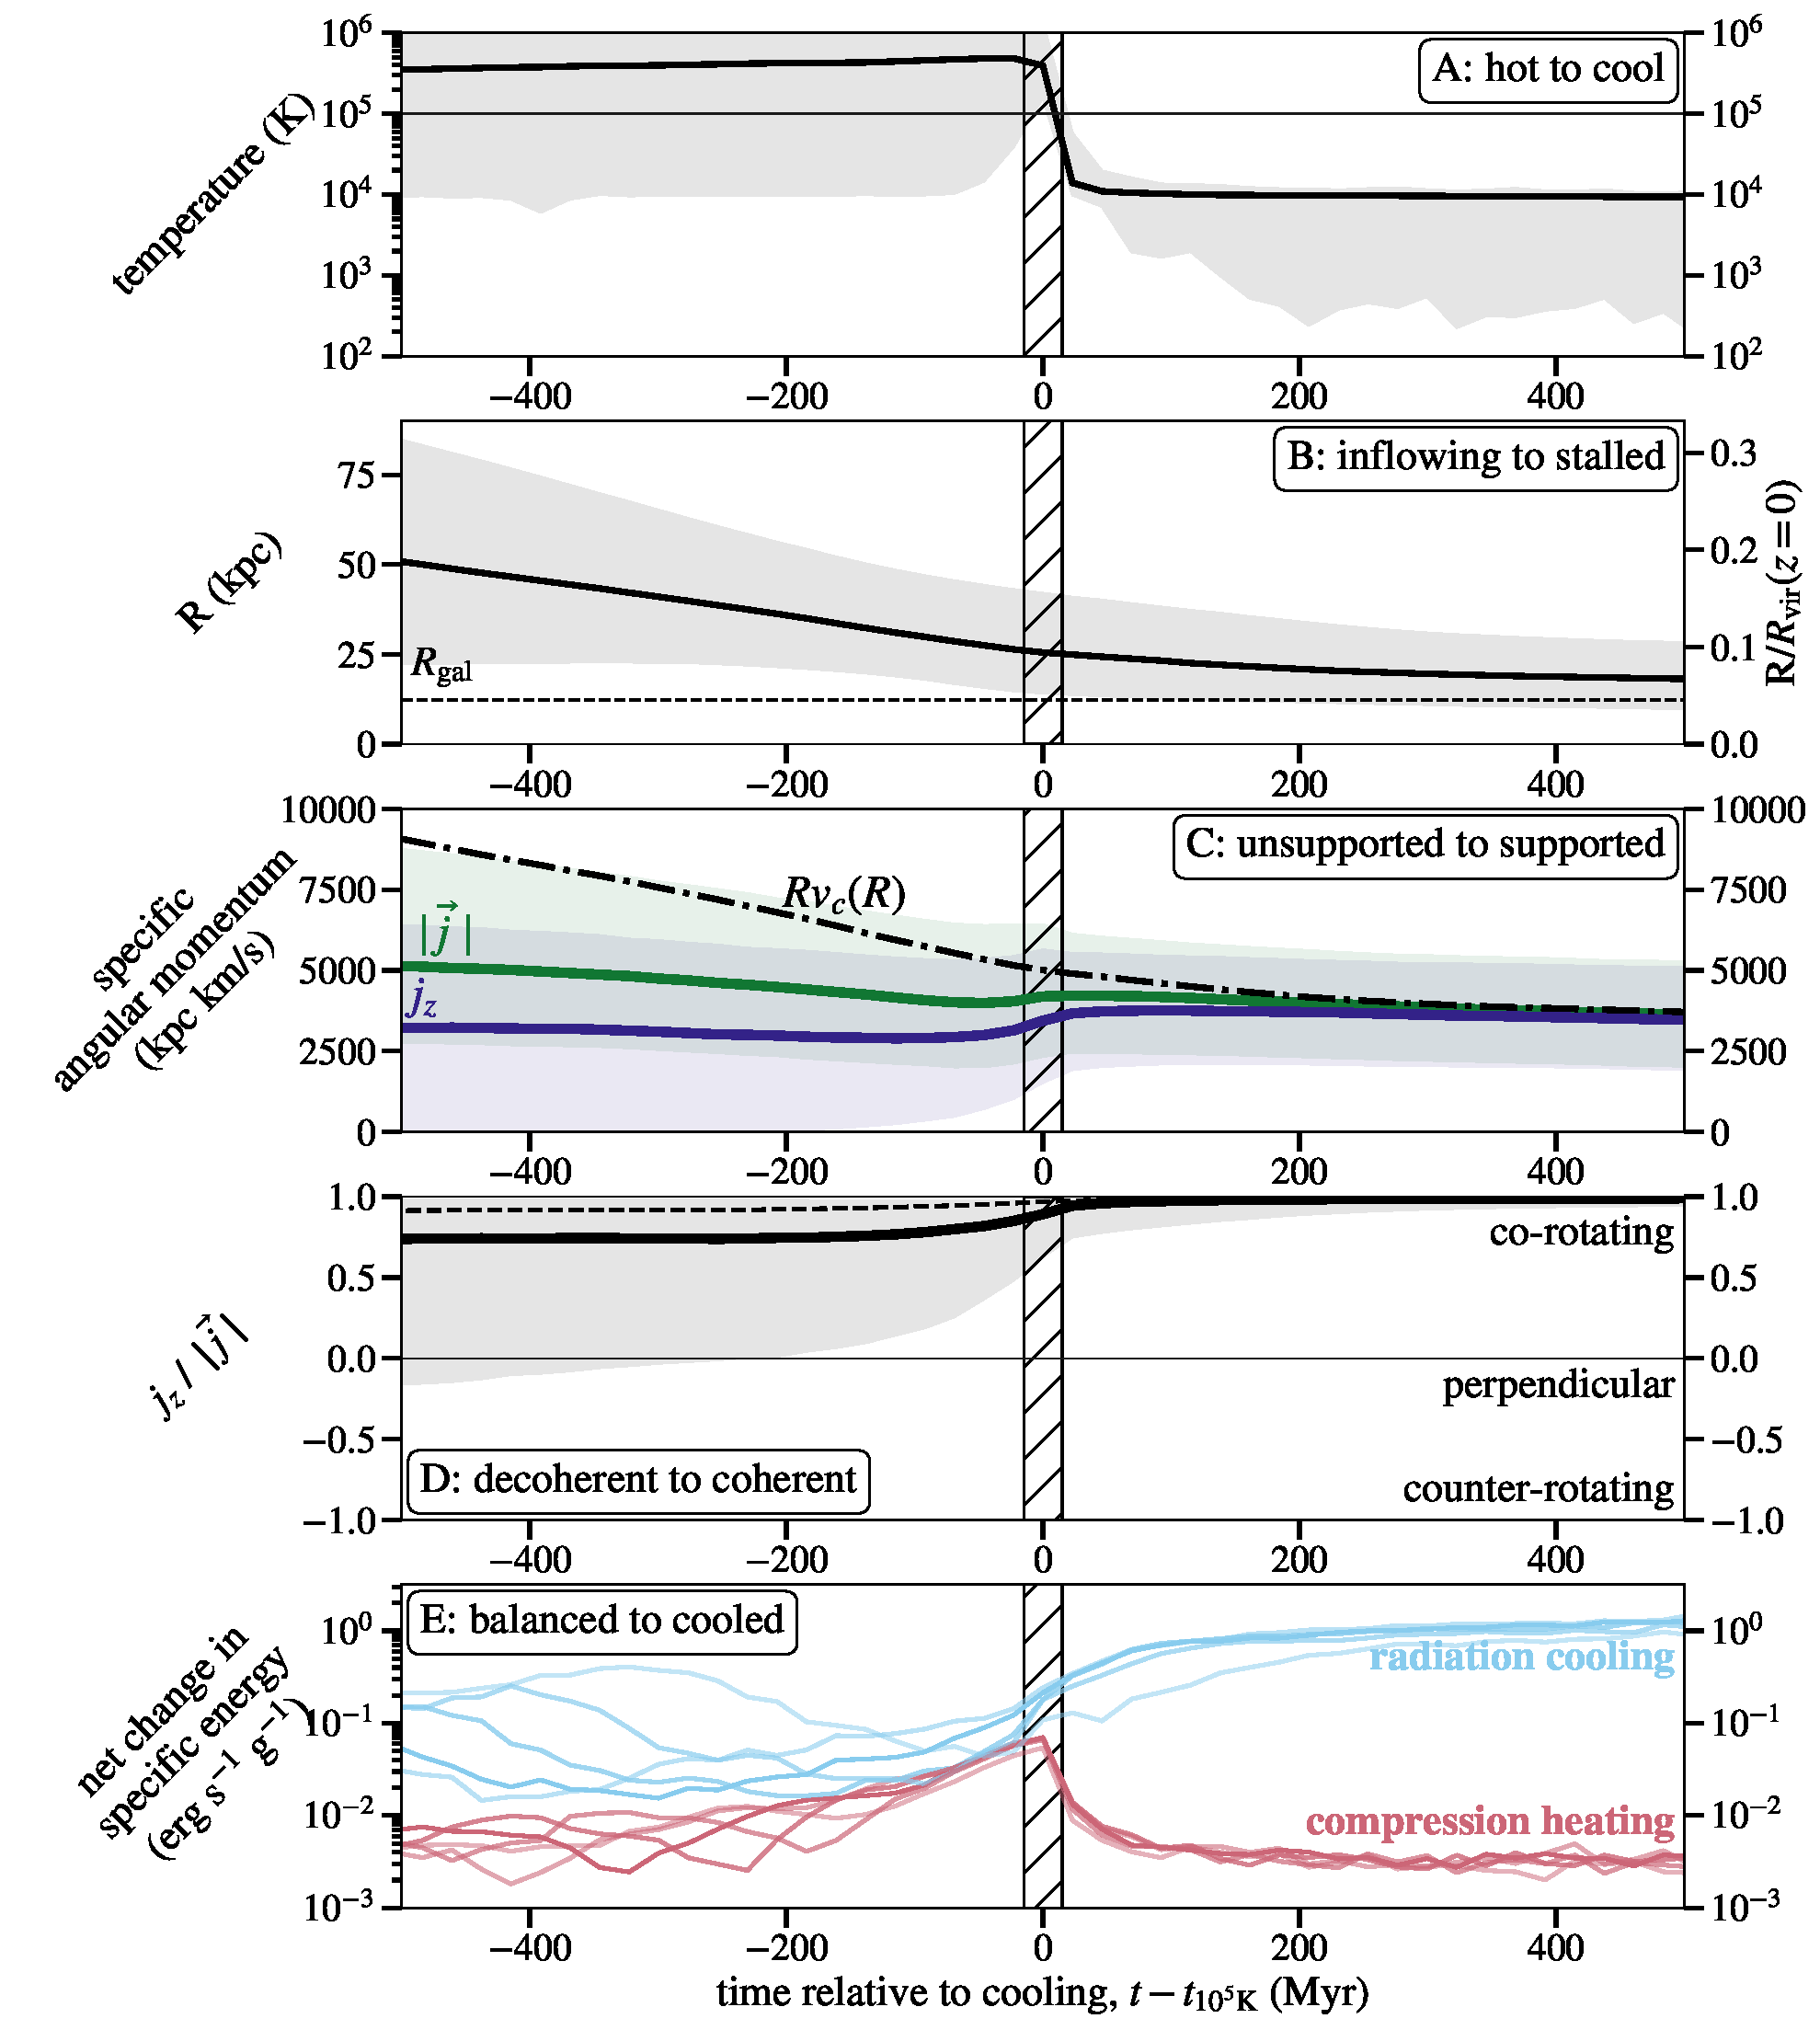
\includegraphics[width=\textwidth]{figures/before_vs_after_cr.pdf}
\caption{
Same as Figure~\ref{f: before and after} but for m12i\_cr.
}
\label{f: before and after cr}
\end{figure*}

\subsection{Metal diffusion vs non-metal diffusion vs MHDCV vs CRs}

\textbf{Plot of distribution $\Rcon$ for m12i and m12i\_md overlapping. Show cooling only happens at large radii in metal diffusion sims.}

\textbf{Add mhdcv comparison.}

\section{Dependence on Deposited Mass}

\begin{figure}
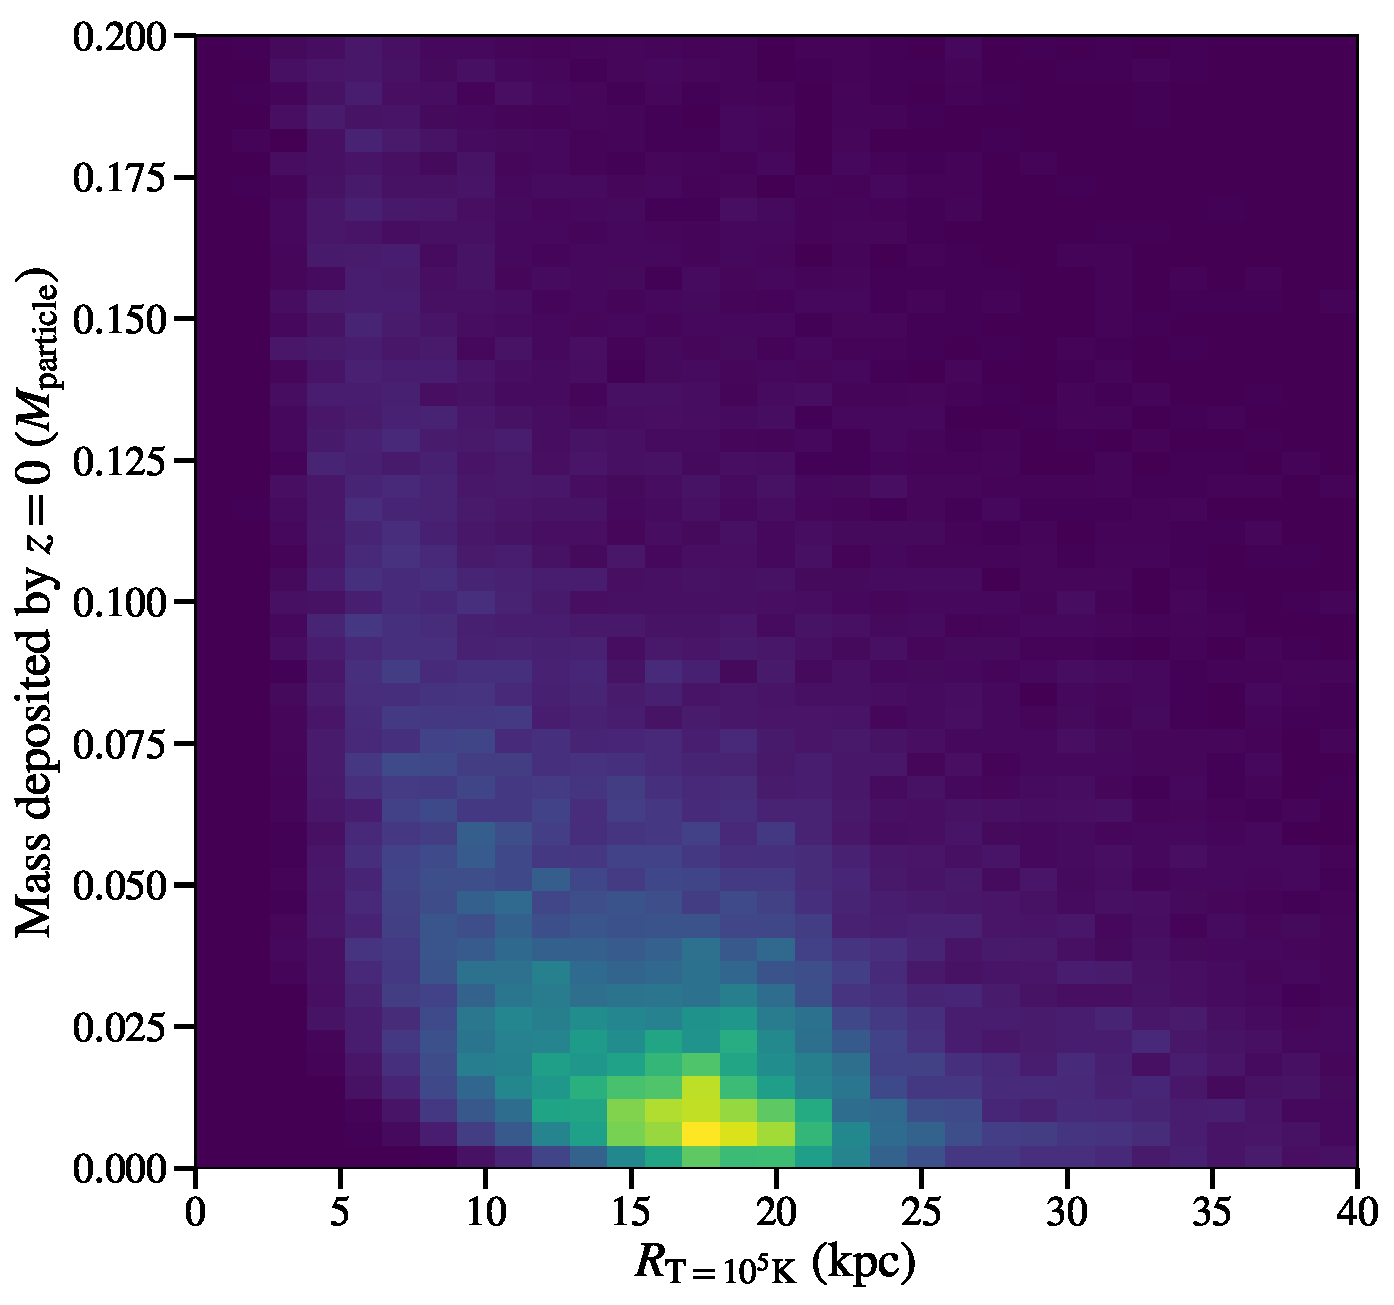
\includegraphics[width=\columnwidth]{figures/mass_dep_vs_R1e5.pdf}
\label{f: deposited mass vs R1e5}
\end{figure}

% \section{Angular Momentum of Accreting Material}

% \begin{figure}
%     \centering
%     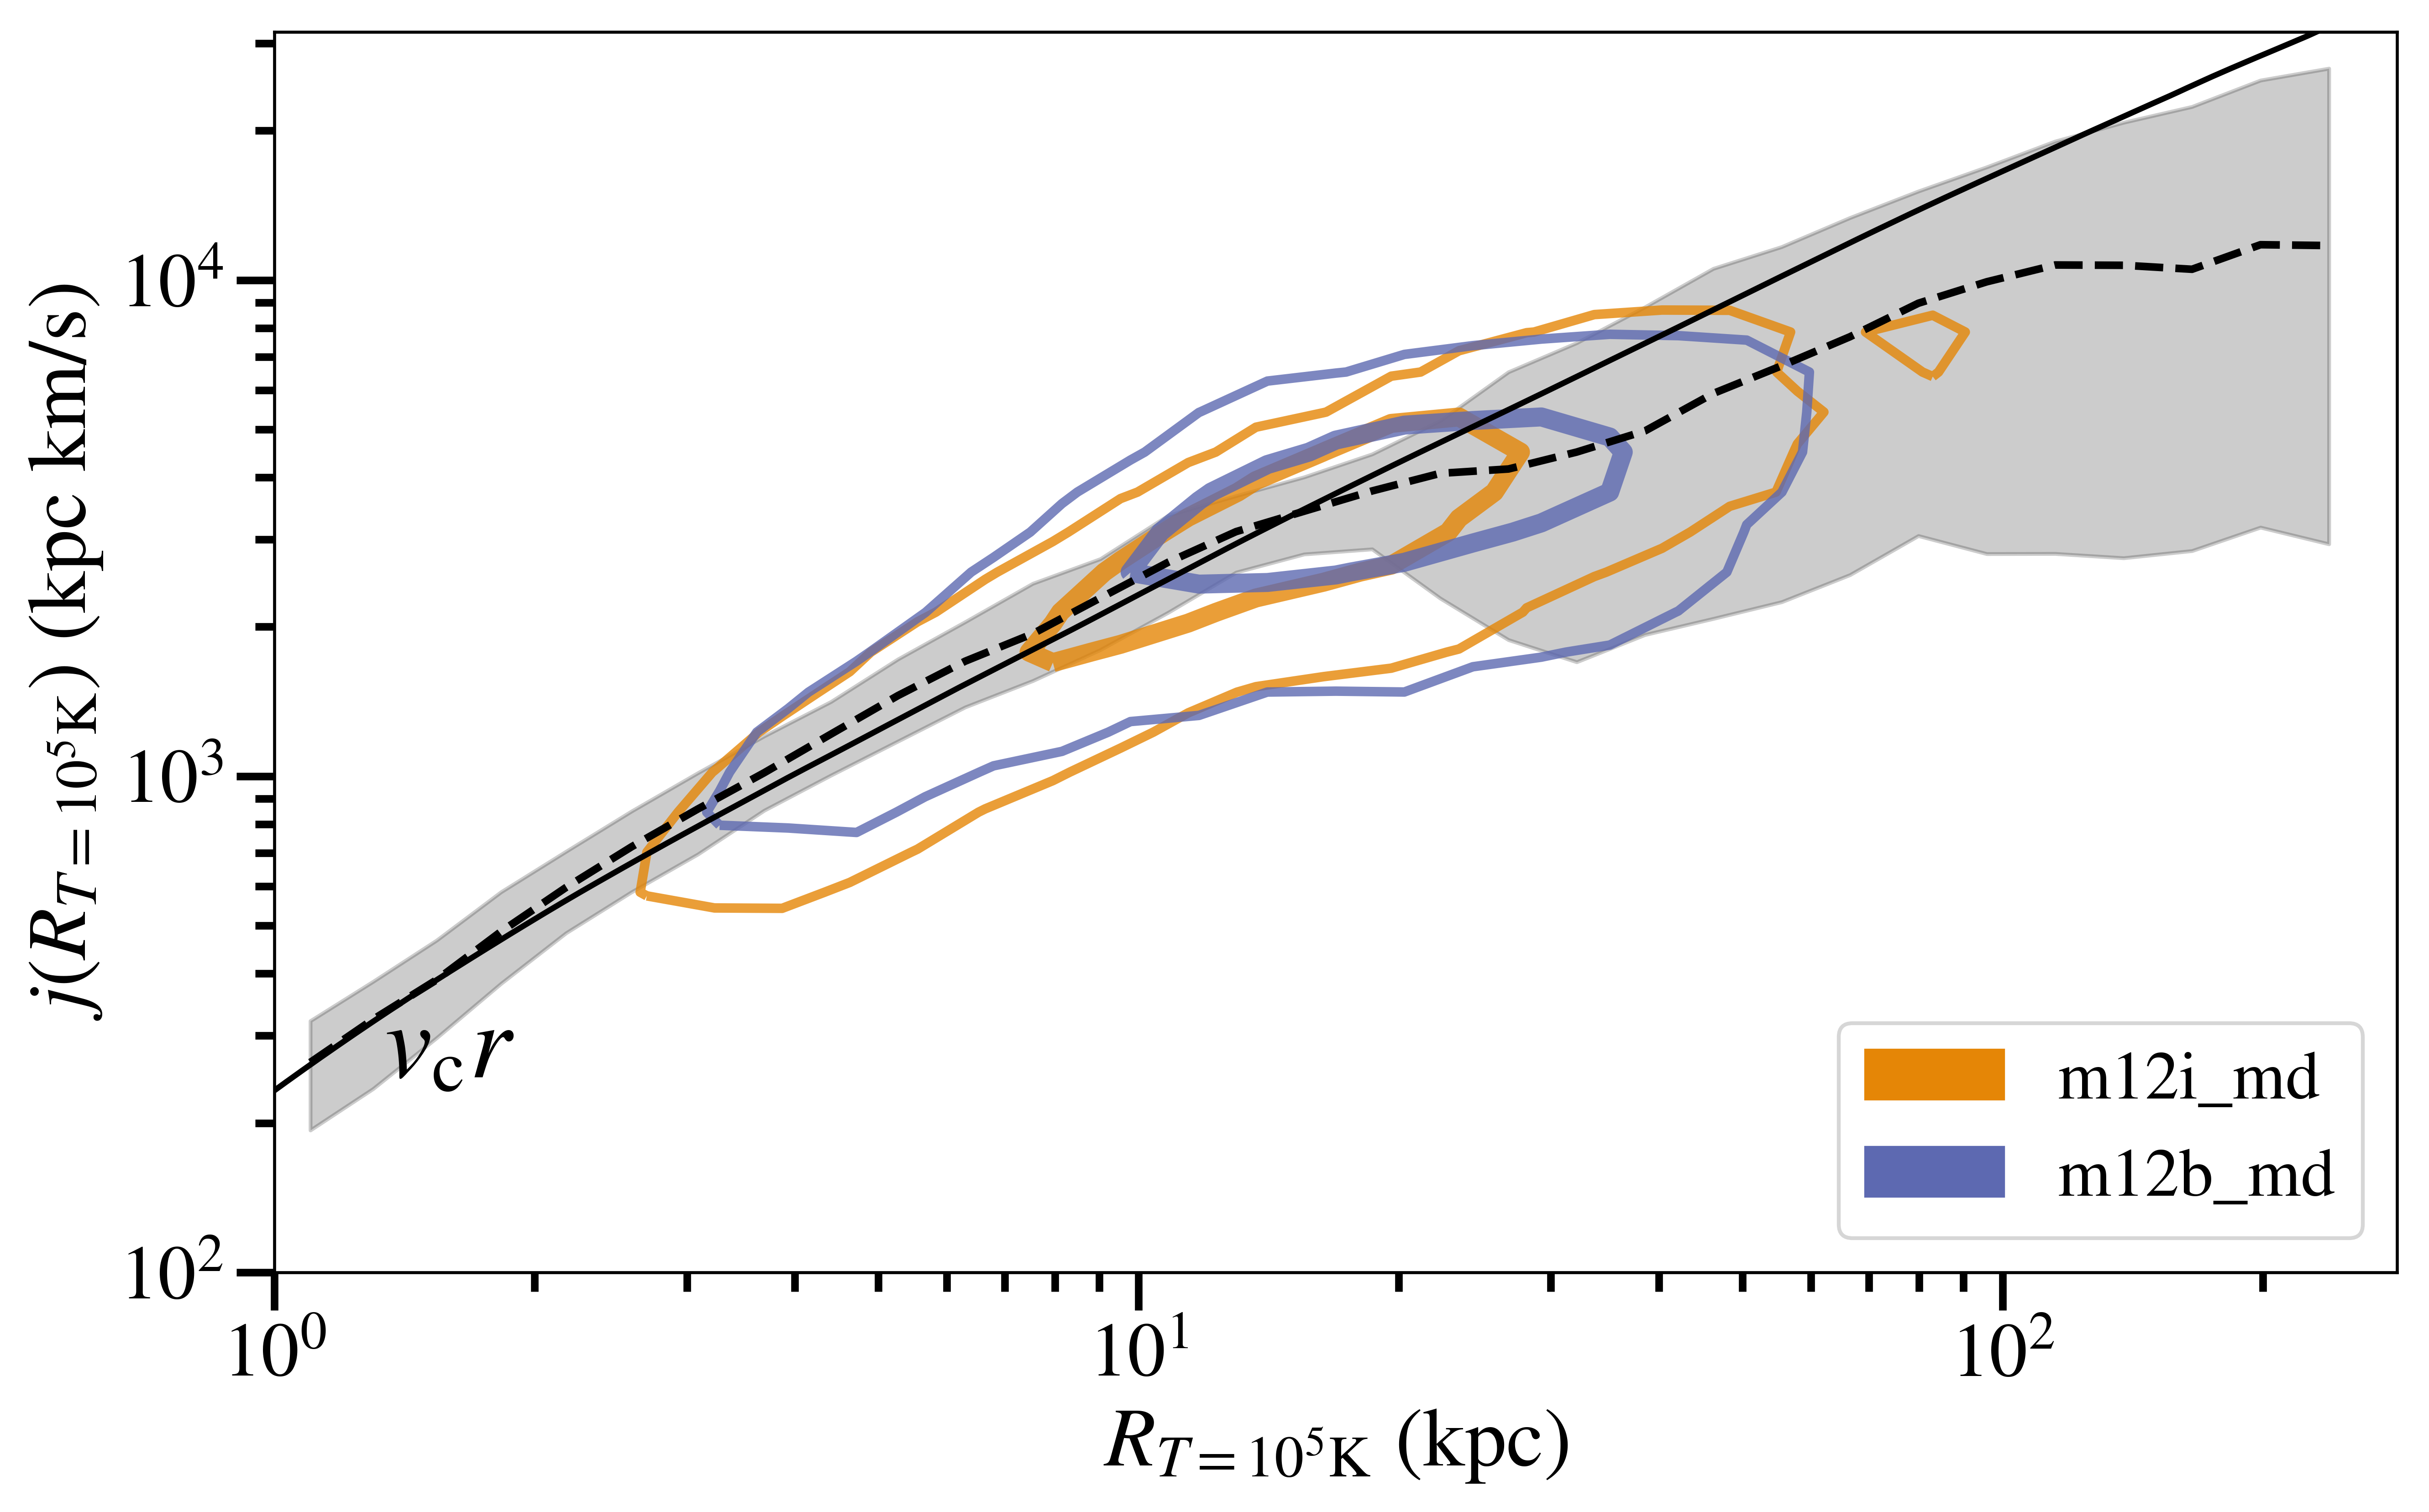
\includegraphics[width=\columnwidth]{figures/j_vs_rcondense.png}
%     \caption{
%     Distribution of $\Rcon$ vs j($\Rcon$) for four FIRE-2 halos with $L(z=0) \sim L^\star$.
% Thick (thin) contours enclose values for 50\% (90\%) of the accreted gas particles.
% The angular momentum as a function of radius for all gas in \texttt{m12i} at $z=0$ is displayed as a dashed line (the median) and shaded regions (5th-95th percentiles).
% \textbf{
% Maybe delete this figure later, because it's only relevant for simulations that have a wide distribution of $\Rcon$, which are only the artificially wide non-md runs.
% }
% \textbf{Is the 100 kpc-cooling gas related to satellite galaxies?}
% \textbf{Try changing shaded region to only hot gas instead of all gas.}
% \textbf{Try histogram of r/(j/vc) instead, to demonstrate that that decreases the spread.}
% \textit{
% In all halos the distributions are consistent with $j_{\rm c} = v_{\rm c} r$, i.e. gas cools once circularized.
% This demonstrates that the variable angular momentum of incoming gas drives the width in the $\Rcon$ distribution.
% }
%     }
%     \label{f: jcool vs Rcon}
% \end{figure}

%%%%%%%%%%%%%%%%%%%%%%%%%%%%%%%%%%%%%%%%%%%%%%%%%%


% Don't change these lines
\bsp	% typesetting comment
\label{lastpage}
\end{document}

% End of mnras_template.tex
